%			PREAMBLE
%
\RequirePackage{ifpdf}
\ifpdf
\documentclass[pdftex,12pt,openright,a4paper,oneside]{book}
\else
\documentclass[12pt,openright,a4paper,oneside]{book}
\fi

\usepackage{graphicx}
\usepackage{url}
\usepackage{xurl}
\usepackage{hyperref}
\usepackage{epsfig}
\usepackage{wrapfig}
\usepackage{lscape}
\usepackage{rotating}
\usepackage{epstopdf}
\usepackage{float}
\usepackage{setspace}
\usepackage{thesis}
\usepackage[round]{natbib}
\usepackage{amssymb,amsmath,amsthm}
\usepackage{bbm}
\usepackage{afterpage}
\usepackage{booktabs}
\usepackage{tabularx}
\usepackage{array}
\usepackage{longtable}
\usepackage{ragged2e}
\usepackage{chngcntr}


% ---(Colors)-------------------------------------------------------------
\ifpdf
\usepackage[pdftex]{color}
\else
\usepackage[dvips]{color}
\fi
% ---(Images)-------------------------------------------------------------
\ifpdf
\DeclareGraphicsExtensions{.pdf,.png,.jpg}
\else
%\usepackage[draft]{graphicx}
\usepackage[dvips]{graphicx}
\DeclareGraphicsExtensions{.eps}
\fi

\newcommand\blankpage{%
    \null
    \thispagestyle{empty}%
    \addtocounter{page}{-1}%
    \newpage}
\bibliographystyle{apalike}

\usepackage[utf8]{inputenc}
%
\newtheorem{myteor}{Teorema}[section]
%
\newenvironment{teor}{\begin{myteor}\sl}{\end{myteor}}

\setlength{\evensidemargin}{0.1cm}
\setlength{\oddsidemargin}{0.6cm}
\setlength{\topmargin}{0cm}
\setlength{\headheight}{0cm}
\setlength{\textheight}{22cm}
\setlength{\topskip}{0cm}
\setlength{\textwidth}{15.4cm}
\setlength{\footskip}{2.3cm}
%\setlength{\footheight}{1cm}
\setlength{\headsep}{1.4\headsep}


\newcommand {\myimage}[4] {
\begin{figure}[ht!]
    \begin{center}
        \includegraphics{#1}
        \caption{\textit{#2}}
        \textit{#3}
        \label{fig:#4}
    \end{center}
\end{figure}
}

\newcommand {\dedicate}[1]{
        \newpage
        \begin{flushright}\large\em\null\vskip1in
        #1
        \vfill\end{flushright}
}
%
%
%			TITLE
%
\begin{document}
\baselineskip=1.5
\normalbaselineskip

\pagestyle{empty}


\title{Thesis Title}
\author{Leila CIELOK}
\dept{Master Degree in Data Science for Economics} 
\anno{2026/2027}
\matricola{65522A}
\relatore{Prof. Luca ROSSINI} %supervisor
\correlatore{Prof. Maria Fernanda PINTADO SERRANO} %co-supervisor

% \afterpage{\blankpage}
% 
%			QUOTE (optional)
%
\beforepreface
% comment if not required
\dedicate{$<$exergo - dedicate$>$}

% \afterpage{\blankpage}
%
%			ACKNOWLEDGMENTS
%
\prefacesection{Aknowledgments}
ACKNOWLEDGMENTS
% \afterpage{\blankpage}

\afterpreface

\chapter*{Abstract}
\label{chap:abstract}
ABSTRACT.
% 
% 
%			CHAPTER 1: Introduction
\chapter{Introduction}
\label{chap:introduction}
Background and Motivation


\section{Research Question}
\label{sec:research_question}
Research problem: identifying how global lng maritime network nodes' criticality evolves in time, distinguishing the probability that a node is active from its criticality conditioned on being active.

1. How will the structure of the global LNG maritime network evolve between 2020 and 2024?

2. What characteristics determine the probability that a terminal or chokepoint will be operational in a given month?

3. Which latent dimensions collectively describe the various measures of criticality?

4. How do structural, infrastructural and dynamic characteristics influence the criticality of nodes?

5. How do the mechanisms of criticality differ between terminals and chokepoints?

\section{Contributions}
\label{sec:contributions}
Empirical (new monthly lng maritime dataset), methodology (separation: activity vs conditional criticality), theoretical (multidimensionality of criticality).

\section{Thesis structure}
\label{sec:thesis_structure}
This thesis is structured as follows...
% 
%			CHAPTER 2: State of the Art
% 
\chapter{Literature review}
\label{chap:soa}

\section{Section 1}
\label{sec:sec_1}
Global LNG Maritime trade networks: LNG organization, description of nodes' roles and routes.

\section{Section 2}
\label{sec:sec_2}
Potential subsections:

Criticality and Vulnerability in network analysis: comparison of importance, centrality, criticality, vulnerability, network science measures' roles.

Dynamic and temporal networks: temporal dependence, nodes inactivity and persistence.

Statistical models for sparse network processes: hurdle models

Bayesian reduced-rank models: multivariate bayesian models, shrinkage\dots

Research gap: combine dynamicity, multidimensional criticality, terminals and chokepoints analysis together

\subsection{Subsection 2.1}
\label{sec:subsec_1}
% 
%
%			CHAPTER 3: Data and network construction
%
\chapter{Data and network construction}
\label{chap:data_network}

This chapter describes the data sources and processing steps used to construct the dynamic LNG maritime network analysed in this thesis. The final dataset combines observed LNG tanker voyages, import and export terminals, reconstructed maritime routes, and the strategic chokepoints traversed by those routes. Together, these components represent the global LNG transportation system as a directed and weighted network evolving at a monthly frequency from January 2020 to December 2024. 

The construction process involved harmonising the source data, matching observed voyages to their departure and arrival terminals, reconstructing the corresponding maritime routes, identifying the chokepoints crossed by each route, and aggregating trade flows and network relationships at the monthly level. The resulting dataset contains the nodes, connections, flow volumes, route characteristics, and infrastructure attributes required for the descriptive and Bayesian analyses developed in the following chapters.

\section{Data sources}
\label{sec:data_sources}
Despite the growing importance of LNG for international energy trade and energy security, publicly available data with high spatial and temporal resolution remain limited. Official and industry sources generally report LNG trade at the country level and at monthly or annual frequencies, whereas more granular information is often available only through commercial databases. Moreover, to the best of my knowledge, no single open-access dataset jointly represents individual LNG voyages, terminal infrastructure, reconstructed maritime routes, and the strategic chokepoints traversed by those routes.

The dataset used in this thesis was therefore constructed by integrating voyage-level LNG trade records and terminal infrastructure data with reconstructed maritime routes and additional geographic information on maritime chokepoints. The following subsections describe the four main components of this integrated dataset.

\subsection{LNG trade and infrastructure data}
\label{subsec:lng_trade_infrastructure}
The main data source is the Liquefied Natural Gas from Tanker, Terminal, and Trade (LNG-T3) dataset developed by \citet{zhou2026}. LNG-T3 is an open-access dataset providing global LNG infrastructure and trade information at daily resolution for the period from January 2020 to December 2024. It was constructed by combining Automatic Identification System (AIS) vessel-position and draught reports, historical port-call records, LNG tanker specifications, and terminal metadata. The complete dataset contains 17,592 individual LNG tanker voyage events and provides information on tanker movements, terminal activity, and country-to-country trade flows.

Two components of LNG-T3 were used directly in this study: the voyage-level records and the terminal inventory. The voyage data form the empirical basis for identifying directed LNG trade connections and measuring the volumes transported between terminals. The terminal inventory defines the infrastructure nodes of the network and provides the geographic and structural attributes used to characterise them. These two components were linked through the terminal identifiers included in the original dataset.

LNG-T3 was preferred to aggregate country-level trade statistics because its voyage-level resolution makes it possible to identify the specific origin and destination terminals associated with each LNG shipment. 
Its 2020--2024 coverage also provides a consistent five-year observation window that captures both established trade patterns and major changes in the global LNG market, including those following the disruption of European gas supplies in 2022.

\subsubsection{LNG voyages}
\label{subsubsec:lng_voyages}
The LNG-T3 voyage data contain individual movements of LNG tankers between departure and arrival terminals. For each voyage, the available information includes the tanker identifier, the origin and destination terminals, the departure and arrival dates, and the estimated volume of LNG transported. These records were used to identify the direction, timing, and magnitude of LNG flows within the network.

Each voyage was represented as a directed movement from its departure terminal to its arrival terminal. The voyage date was then used to assign the observation to a monthly period between January 2020 and December 2024. When multiple voyages occurred between the same origin--destination pair during the same month, their transported volumes were aggregated. The resulting monthly observations define the directed and weighted trade connections between terminal nodes.

Voyage identifiers were also used to retain information on the number of shipments associated with each connection. This makes it possible to distinguish between connections characterised by a small number of high-volume voyages and those supported by more frequent tanker movements. Once the corresponding maritime routes had been reconstructed, route distance and chokepoint crossings were linked back to the individual voyage records and subsequently aggregated at the monthly level.

\subsubsection{LNG terminals}
\label{subsubsec:lng_terminals}
The LNG-T3 terminal inventory provides the identifiers, names, geographic coordinates, countries, and infrastructure characteristics of LNG facilities worldwide. Terminals constitute the origin and destination nodes of the trade network and were linked to the voyage records using their unique identifiers.

The infrastructure attributes retained for the analysis include the terminal's country, infrastructure type, processing capacity, number of infrastructure units, and start year. Infrastructure type distinguishes facilities according to their import or export function, while capacity provides an indicator of their potential scale of operation. The number of infrastructure units supplies an additional measure of facility size and complexity. The start year was used to construct terminal age as a time-varying variable, calculated for each monthly observation as the difference between the observation year and the year in which the terminal began operating.

Terminal coordinates were used both to position terminal nodes geographically and to reconstruct the maritime route associated with each observed origin--destination pair. Before route reconstruction, terminal identifiers and coordinates were checked for consistency across the voyage and infrastructure data. This harmonisation ensured that every retained voyage could be linked to a valid departure terminal and arrival terminal.

\subsection{Maritime routes and chokepoint data}
\label{subsec:routes_chokepoints_data}
While the LNG-T3 voyage records identify the origin and destination of each shipment, they do not provide the actual maritime path connecting the two terminals. 
For this reason, maritime routes were reconstructed from the geographic coordinates of the departure and arrival terminals using the \texttt{SeaRoute} routing software \citep{searoute}. 

\subsubsection{SeaRoute software}
\label{subsubsec:searoute_software}
SeaRoute applies Dijkstra's algorithm \citep{dijkstra1959} to identify the shortest path between two locations on a predefined network representing frequently used shipping lanes, which accounts for coastlines, navigable waterways, and supported maritime passages.
Specifically, the 5-km resolution of the maritime network produced through the \texttt{marnet} module was used: edges shorter than this scale are progressively contracted and geometrically similar connections are removed, reducing network complexity while preserving the principal maritime routes.
Additionally, in line with the thesis' objectives, transit through both the Suez and Panama canals was enabled, allowing the routing algorithm to include these passages when they formed part of the shortest available maritime path.

Rather than reconstructing the same route separately for every voyage, a route was generated for each unique origin--destination terminal pair and subsequently linked to all voyages associated with that pair. 
The reconstructed routes were subsequently merged with the chokepoints locations to identify the strategic maritime passages traversed by each trade connection.

\subsubsection{Chokepoints geometries}
\label{subsubsec:chokepoints_geom}
The initial set of 28 maritime chokepoints, together with their names, identifiers, and reference coordinates, was obtained from the IMF PortWatch chokepoint database \citep{imf_portwatch}, but because the PortWatch locations are represented primarily as point features, they could not be used directly to determine whether a reconstructed maritime route effectively crossed a passage.
A geometry registry was therefore compiled to associate each chokepoint with an appropriate spatial representation and to document its source and construction method.

The final geometries were assembled from several sources. Published polygons for the Suez Canal, Bab el-Mandeb Strait, and Cape of Good Hope were directly obtained from the World Bank Development Data Partnership's Red Sea Monitoring project \citep{worldbank_redsea}. 
Detailed IHO or SeaVoX geometries for the Malacca, Hormuz, Gibraltar, Dover, and Makassar straits were obtained through the Marine Regions Gazetteer and its geospatial services \citep{marine_regions}. 
For the Lombok, Sunda, Torres, and Bering straits, transit geometries were reconstructed from the WGS84 coordinates reported in official International Maritime Organization routeing documents \citep{imo_colreg74, imo_sn1_326, imo_bering_routeing}. 

Where no suitable published polygon was available, operational geometries were constructed specifically using either a buffered centreline, as in the Panama Canal and Bosporus Strait, or an oriented crossing gate positioned across the relevant navigable passage. 
The placement of these geometries was informed by the reference coordinates provided by PortWatch \citep{imf_portwatch}, geographic information from Marine Regions \citep{marine_regions}, and navigational references from relevant IMO
documents, the NGA GeoNames database, and NOAA/NCEI hydrographic survey records \citep{imo_msc72_69,nga_geonames,noaa_h01600a}.

As a final step, all geometries were transformed into a common geographic coordinate system and stored in a harmonised geospatial format. 
To accommodate small discrepancies between the reconstructed \texttt{SeaRoute} paths and the operational chokepoint geometries, a uniform spatial-tolerance buffer of 25~km was applied around each chokepoint geometry. 
A reconstructed origin--destination route was classified as traversing a chokepoint when it intersected the corresponding buffered geometry.
Of the 28 candidate chokepoints, 24 were traversed by at least one reconstructed route under the final 25-km specification and were therefore retained as nodes in the monthly network.

The robustness of the route--chokepoint assignments was assessed by comparing the final 25-km specification with exact geometric intersection and with alternative buffers of 5 and 10~km. 
The complete sensitivity analysis is reported in Appendix~\ref{app:chokepoint_sensitivity}.

The source, geometry type, construction method, and relevant parameters associated with each of the 28 chokepoints are documented in the geometry registry.

Table~\ref{tab:data_sources} summarises the principal data sources, their units of observation, the main variables retained, and their role in the construction of the network.

\begin{table}[H] 
    \centering 
    \caption{Summary of data sources} 
    \label{tab:data_sources} 
    \small 
    \begin{tabularx}{\textwidth}{ 
        >{\raggedright\arraybackslash}p{0.18\textwidth} 
        >{\raggedright\arraybackslash}p{0.15\textwidth} 
        >{\raggedright\arraybackslash}X 
        >{\raggedright\arraybackslash}X 
    } 
        \toprule 
        \textbf{Source} & 
        \textbf{Unit of observation} & 
        \textbf{Main variables} & 
        \textbf{Role in the analysis} \\ 
        \midrule 
        
        LNG-T3 tanker voyages & 
        Individual voyage & 
        Departure and arrival terminals, voyage dates, tanker identifier, estimated LNG volume & 
        Identification of directed LNG trade connections and monthly flow volumes from January 2020 to December 2024\\ 
        \addlinespace 
        
        LNG-T3 terminal inventory & 
        LNG terminal & 
        Terminal identifier, name, coordinates, country, infrastructure type, capacity, unit count, start year & 
        Definition and characterisation of terminal nodes \\ 
        \addlinespace 
        
        \texttt{searoute} & 
        Unique origin--destination pair & 
        Reconstructed maritime path, route distance & 
        Reconstruction of the geographic route associated with each trade connection \\ 
        \addlinespace 
        
        Chokepoint geographic data & 
        Maritime chokepoint & 
        Name, type, and geographic location & 
        Definition of chokepoint nodes, identification of route crossings \\ 
        \bottomrule 
    \end{tabularx} 
\end{table}

\section{Data preparation}
\label{sec:data_preparation}
Before constructing the network, the voyage and terminal datasets were harmonised to ensure that each observed shipment could be associated with a unique origin and destination node. 
This harmonization process began by converting date fields and numerical variables into consistent formats as an initial validation step, followed by the parsing of all voyage dates, LNG volumes, terminal capacities, and unit counts, with no invalid non-missing values detected. 
Start year was unavailable for 64 of the 545 records in the original terminal inventory, although this information was complete for all 159 terminals subsequently retained in the network.

The LNG-T3 terminal inventory contains 545 records corresponding to 471 unique terminal names. Sixty-five terminal names appear more than once, reflecting different infrastructure-status records for the same facility. Most repeated records report identical coordinates, whereas three terminal names are associated with two distinct coordinate variants each. To construct a unique terminal map, distinct name--coordinate combinations were initially assigned separate identifiers, while records sharing both terminal name and coordinates were treated as referring to the same facility.

A canonical record was then selected for each terminal name using the infrastructure status reported in the original dataset, with priority given to operating facilities, followed by facilities under construction, idle, mothballed, and proposed. 
The coordinate variants associated with the three affected terminal names were retained in a separate validation table, together with an indicator identifying the variant selected as canonical. 
Each of the resulting 471 terminal records was assigned a unique node identifier.

Voyage origins and destinations were matched to the consolidated terminal map using the terminal names reported in the LNG-T3 voyage data. 
The corresponding node identifiers and coordinates were attached to each voyage record, and the matching status of the two endpoints was recorded separately. 
All origin and destination values in the 17,592 voyage records were successfully matched to the terminal map.

The original voyage table contains 8,645 laden export voyages and 8,947 return movements, with all return movements reporting zero transported LNG volume and therefore being excluded from the trade network. 
The retained records were additionally required to have a valid departure date, matched origin and destination identifiers, and a strictly positive LNG volume. 
All export records satisfied these conditions, meaning that these checks did not produce any further exclusions.

Potential duplicate export observations were identified using the departure and arrival dates, tanker IMO number, voyage type, origin and destination terminals, and transported volume. 
Five rows belonged to two duplicate groups: one voyage appeared twice and another appeared three times. 
Retaining the first observation in each group removed three duplicate rows. The final dataset used to construct the network therefore contains 8,642 laden LNG voyages.

\subsection{Terminal infrastructure characteristics}
\label{subsec:terminal_roles_characteristics}
Terminal characteristics were obtained from the LNG-T3 infrastructure inventory and linked to the consolidated terminal identifiers. 
The retained attributes include country, region, geographic coordinates, infrastructure type, operational status, annual processing capacity, number of infrastructure units, and start year. 
No missing values were found for these attributes among the terminals retained in the final network.

Additionally, terminal age was constructed as a time-varying characteristic by subtracting the terminal's reported start year from the year of each monthly observation:

\begin{equation}
\operatorname{Age}_{i,t}
=
\operatorname{Year}_{t}
-
\operatorname{StartYear}_{i}.
\label{eq:terminal_age}
\end{equation}

\subsection{Temporal aggregation}
\label{subsec:temporal_aggregation}
Each retained voyage was assigned to a monthly period according to its departure date. 
The resulting observation window extends from January 2020 to December 2024, corresponding to the complete five-year coverage of the LNG-T3 dataset and yielding 60 monthly network observations. 

To preserve months in which a node had no observed activity, complete node--month panels were subsequently constructed by combining every retained node with all 60 monthly periods. 
Flow and voyage measures for node--month observations with no activity were assigned a value of zero to distinguish these structural zeros from missing or non-applicable node characteristics, which remained coded as unavailable.

\section{Dynamic network construction} 
\label{sec:dynamic_network_construction} 
The global LNG maritime network was represented as a sequence of monthly directed and weighted graphs, 

\begin{equation} 
    G_t = (V,E_t,W_t), \qquad t=1,\ldots,60, 
    \label{eq:dynamic_network} 
\end{equation}

where \(V\) is the time-invariant set of terminal and chokepoint nodes, \(E_t\) is the set of directed connections observed in month \(t\), and \(W_t=[w_{ij,t}]\) is the corresponding weighted adjacency matrix. 
An element \(w_{ij,t}>0\) represents the total LNG volume transported from node \(i\) to node \(j\) during month \(t\), while \(w_{ij,t}=0\) indicates that no such connection was observed.

\subsection{Nodes and edges} 
\label{subsec:nodes_edges} 
The final node set contains 183 nodes and can be written as 

\begin{equation} 
    V = V^{T} \cup V^{C}, \qquad |V^{T}|=159, \qquad |V^{C}|=24, 
\end{equation}

where \(V^{T}\) denotes the set of LNG terminals and \(V^{C}\) the set of maritime chokepoints. 
The 159 terminal nodes are the facilities that appear as an origin or destination of at least one retained laden voyage. 
Of the 28 candidate chokepoints included in the geographic registry, 24 were traversed by at least one reconstructed route and were therefore retained in the observed network.

Each commercial voyage defines an underlying directed movement from an export terminal to an import terminal. 
To incorporate the maritime infrastructure traversed during transportation, the reconstructed route of voyage \(r\) was represented as an ordered path 

\begin{equation} 
    P_r = \left( v_{r,0},v_{r,1},\ldots,v_{r,K_r} \right), 
\end{equation}

where \(v_{r,0}\) is the departure terminal, \(v_{r,K_r}\) is the arrival terminal, and any intermediate nodes are the chokepoints crossed by the route. 
The voyage was then expanded into the consecutive directed connections

\begin{equation} 
    (v_{r,0},v_{r,1}), (v_{r,1},v_{r,2}), \ldots, (v_{r,K_r-1},v_{r,K_r}). 
\end{equation} 

A route that crossed no retained chokepoint generated a direct terminal-to-terminal edge. 
Routes crossing one or more chokepoints generated terminal-to-chokepoint, chokepoint-to-chokepoint, and chokepoint-to-terminal edges according to the order in which those nodes were encountered.

Let \(\mathcal{R}_t\) denote the set of voyages assigned to month \(t\), \(q_r\) the LNG volume transported by voyage \(r\), and \(\mathcal{E}(P_r)\) the set of consecutive directed connections in its ordered path. 
Monthly edge weights were defined as

\begin{equation} 
    w_{ij,t} = \sum_{r\in\mathcal{R}_t} q_r\, 
    \mathbb{I} \left\{ (i,j)\in\mathcal{E}(P_r) \right\}, 
    \label{eq:monthly_edge_weight} 
\end{equation}

where \(\mathbb{I}\{\cdot\}\) is the indicator function. 
Thus, the full volume of a shipment was assigned to every segment traversed by its route.
Because shipments crossing multiple segments would consequently be counted more than once in the sum of all edge weights, aggregate monthly trade volume was calculated directly from the original voyage observations.

Voyages sharing the same directed pair of nodes within a month were aggregated into a single edge. 
In addition to LNG volume, each monthly edge records the number of voyage traversals, the number of distinct origin--destination routes using the connection, and their route identifiers.

\subsection{Node activity} 
\label{subsec:node_activity_definition} 
Node activity was defined from the presence of incident flow in each monthly graph. 
For node \(i\) in month \(t\), the binary activity indicator was defined as

\begin{equation} 
    a_{i,t} = \mathbb{I} \left\{ \sum_{j\in V} w_{ij,t} + \sum_{j\in V} w_{ji,t} > 0 \right\}. 
    \label{eq:node_activity} 
\end{equation} 

A terminal was therefore classified as active when it recorded positive incoming or outgoing LNG flow during the month. 
Since terminal direction was fully consistent with the infrastructure classification reported in LNG-T3, active export terminals recorded outgoing flow and active import terminals recorded incoming flow. 

A chokepoint was classified as active when at least one voyage traversed it during the month, generating positive incident flow on one or more adjacent route segments. 
Chokepoints not traversed by any voyage in a given month were retained in the balanced node--month panel and assigned an activity value of zero.

\section{Construction of node-level measures}
\label{sec:node_level_measures}

A set of monthly node-level measures was constructed to represent different dimensions of criticality in the LNG transportation network. 
Since terminals and chokepoints perform different functions, their criticality was evaluated using separate but complementary measures and network representations.

On the one hand, terminals represent the origins and destinations of commercial LNG flows. 
Their criticality was therefore defined in terms of their importance as suppliers or recipients, the concentration of their trading relationships, and the dependence associated with those relationships. 
On the other hand, chokepoints represent intermediate passages along maritime routes, and their criticality was consequently defined in terms of their position within the physical transportation network, the volume of LNG passing through them, and their role in connecting otherwise separated parts of the network or in mediating important transportation paths.

Terminal criticality measures were calculated from the original terminal-to-terminal voyage flows, thereby preserving the direct commercial relationship between origins and destinations and avoiding the repeated counting of shipments across multiple route segments. 
Chokepoint criticality measures were instead calculated on the complete segment-level network, including both terminals and chokepoints, so that the position of each passage within the full sequence of maritime movements could be represented. 
Additional structural indicators were calculated for both node types.

\subsection{Terminal criticality measures}
\label{subsec:terminal_measures}
Terminal criticality was represented through measures of directional network importance, counterparty concentration, trade dependence, and voyage distance. 
These measures were constructed monthly and, where relevant, adapted to the terminal's observed role as an LNG exporter or importer.

\subsubsection{Terminal role}
Let \(q_{ij,t}\) denote the total LNG volume transported from terminal \(i\) to terminal \(j\) during month \(t\). 
Monthly outgoing flow, incoming flow, and throughput were defined as

\begin{equation}
\begin{aligned}
O_{i,t} &= \sum_j q_{ij,t}, \\
I_{i,t} &= \sum_j q_{ji,t}, \\
T_{i,t} &= O_{i,t}+I_{i,t}.
\end{aligned}
\label{eq:terminal_flows}
\end{equation}

A terminal was classified as active in month \(t\) when \(T_{i,t}>0\). Among active terminals, the observed monthly role was classified as exporter when \(O_{i,t}>0\) and \(I_{i,t}=0\), importer when \(I_{i,t}>0\) and \(O_{i,t}=0\), and bidirectional when both flows were positive.

For active terminal--months, export share was defined as

\begin{equation}
s^{\mathrm{out}}_{i,t}
=
\frac{O_{i,t}}{T_{i,t}},
\label{eq:export_share}
\end{equation}

so that exporters have \(s^{\mathrm{out}}_{i,t}=1\), importers have \(s^{\mathrm{out}}_{i,t}=0\), and bidirectional terminals take values between zero and one.

\subsubsection{Counterparty concentration}
\label{hhi_index}
The concentration of a terminal's trade across its counterparties was measured using the Herfindahl--Hirschman Index (HHI), a standard measure of concentration based on the squared shares of individual counterparties \citep{hirschman1945}. 
The outgoing and incoming terminal-level concentration indices were calculated, respectively, as

\begin{equation}
\begin{aligned}
H^{\mathrm{out}}_{i,t}
&=
\sum_j
\left(
\frac{q_{ij,t}}{O_{i,t}}
\right)^2, \\
H^{\mathrm{in}}_{i,t}
&=
\sum_j
\left(
\frac{q_{ji,t}}{I_{i,t}}
\right)^2.
\end{aligned}
\label{eq:terminal_hhi}
\end{equation}

The same procedure was applied after aggregating counterparties by country, producing corresponding country-level concentration indices. 
Values approaching one indicate that flows are concentrated in a small number of counterparties, whereas lower values indicate greater diversification.

A role-specific concentration measure was then assigned according to the terminal's observed direction of trade:

\begin{equation}
H^{\mathrm{role}}_{i,t}
=
\begin{cases}
H^{\mathrm{out}}_{i,t},
& \text{if } O_{i,t}>0 \text{ and } I_{i,t}=0, \\[4pt]
H^{\mathrm{in}}_{i,t},
& \text{if } I_{i,t}>0 \text{ and } O_{i,t}=0, \\[4pt]
s^{\mathrm{out}}_{i,t}H^{\mathrm{out}}_{i,t}
+
\left(1-s^{\mathrm{out}}_{i,t}\right)H^{\mathrm{in}}_{i,t},
& \text{if } O_{i,t}>0 \text{ and } I_{i,t}>0.
\end{cases}
\label{eq:role_hhi}
\end{equation}

\subsubsection{Directional PageRank}
\label{subsubsec:directional_pagerank}
Terminal network importance was measured using PageRank, which considers both the magnitude of a terminal's connections and the importance of the terminals to which it is connected \citep{page1999pagerank}. 
The measure was calculated separately for importing and exporting roles on the monthly directed and flow-weighted terminal network: import PageRank was calculated using the observed direction of LNG flows, whereas export PageRank was calculated after reversing all edges. 
Intuitively, import PageRank assigns greater importance to terminals receiving flows from other important terminals, while export PageRank captures the corresponding importance of LNG suppliers.

For the observed network, weighted import PageRank satisfies

\begin{equation}
PR^{\mathrm{imp}}_{i,t}
=
\frac{1-\alpha}{N_t}
+
\alpha
\sum_{\substack{j \\ (j,i)\in E_t}}
PR^{\mathrm{imp}}_{j,t}
\frac{q_{ji,t}}
{\sum_k q_{jk,t}},
\label{eq:import_pagerank}
\end{equation}

where \(N_t\) is the number of active terminals in month \(t\), and the damping factor was set to \(\alpha=0.85\). Export PageRank, \(PR^{\mathrm{exp}}_{i,t}\), was obtained by applying the same calculation to the reversed monthly network.

The role-specific PageRank measure was defined as

\begin{equation}
PR^{\mathrm{role}}_{i,t}
=
\begin{cases}
PR^{\mathrm{exp}}_{i,t},
& \text{if } O_{i,t}>0 \text{ and } I_{i,t}=0, \\[4pt]
PR^{\mathrm{imp}}_{i,t},
& \text{if } I_{i,t}>0 \text{ and } O_{i,t}=0, \\[4pt]
s^{\mathrm{out}}_{i,t}PR^{\mathrm{exp}}_{i,t}
+
\left(1-s^{\mathrm{out}}_{i,t}\right)
PR^{\mathrm{imp}}_{i,t},
& \text{if } O_{i,t}>0 \text{ and } I_{i,t}>0.
\end{cases}
\label{eq:role_pagerank}
\end{equation}

\subsubsection{Trade dependence}

For each directed terminal pair, the dependence of an importing terminal \(j\) on an exporter \(i\) was measured as the share of \(j\)'s total imports supplied by \(i\):

\begin{equation}
d_{ij,t}
=
\frac{q_{ij,t}}{I_{j,t}}.
\label{eq:recipient_dependence}
\end{equation}

To summarise the dependence generated by exporter \(i\), this bilateral measure was weighted by the share of the exporter's flow directed towards each destination:

\begin{equation}
D^{\mathrm{exp}}_{i,t}
=
\sum_j
\left(
\frac{q_{ij,t}}{O_{i,t}}
\right)
d_{ij,t}.
\label{eq:export_dependence}
\end{equation}

The resulting measure is high when an exporter directs a substantial share of its LNG towards terminals that depend strongly on its supply.

For an importing terminal \(i\) located in country \(c(i)\), dependence was measured as its share of the total LNG volume received by all terminals in that country:

\begin{equation}
D^{\mathrm{imp}}_{i,t}
=
\frac{I_{i,t}}
{\displaystyle\sum_{k:\,c(k)=c(i)} I_{k,t}}.
\label{eq:import_dependence}
\end{equation}

The role-specific dependence measure was subsequently defined as

\begin{equation}
D^{\mathrm{role}}_{i,t}
=
\begin{cases}
D^{\mathrm{exp}}_{i,t},
& \text{if } O_{i,t}>0 \text{ and } I_{i,t}=0, \\[4pt]
D^{\mathrm{imp}}_{i,t},
& \text{if } I_{i,t}>0 \text{ and } O_{i,t}=0, \\[4pt]
s^{\mathrm{out}}_{i,t}D^{\mathrm{exp}}_{i,t}
+
\left(1-s^{\mathrm{out}}_{i,t}\right)
D^{\mathrm{imp}}_{i,t},
& \text{if } O_{i,t}>0 \text{ and } I_{i,t}>0.
\end{cases}
\label{eq:role_dependence}
\end{equation}

\subsubsection{Mean voyage distance}

Mean voyage distance was calculated as the unweighted arithmetic mean of the reconstructed distances of voyages associated with each terminal. For an exporting terminal, this corresponds to

\begin{equation}
\overline{L}^{\mathrm{out}}_{i,t}
=
\frac{1}{n^{\mathrm{out}}_{i,t}}
\sum_{r\in\mathcal{R}^{\mathrm{out}}_{i,t}} L_r,
\label{eq:outgoing_distance}
\end{equation}

where \(\mathcal{R}^{\mathrm{out}}_{i,t}\) is the set of voyages departing from terminal \(i\) in month \(t\), \(n^{\mathrm{out}}_{i,t}\) is their number, and \(L_r\) is the reconstructed distance of voyage \(r\).

For an importing terminal, the corresponding measure was defined as

\begin{equation}
\overline{L}^{\mathrm{in}}_{i,t}
=
\frac{1}{n^{\mathrm{in}}_{i,t}}
\sum_{r\in\mathcal{R}^{\mathrm{in}}_{i,t}} L_r,
\label{eq:incoming_distance}
\end{equation}

where \(\mathcal{R}^{\mathrm{in}}_{i,t}\) is the set of voyages arriving at terminal \(i\) in month \(t\). The role-relevant mean voyage distance was subsequently lagged by one month before being included among the model covariates.

\subsection{Chokepoint criticality measures}
\label{subsec:chokepoint_measures}
Chokepoint criticality was represented through weighted betweenness, PageRank, and the share of monthly network flow. Together, these measures capture complementary dimensions of a passage's importance, including its position along high-flow paths, its centrality in the direction of LNG movement, and the volume of LNG transported through it.

\subsubsection{Weighted betweenness centrality}
Betweenness centrality measures the extent to which a node lies on shortest paths between other nodes \citep{brandes2001}. 
Since edge weights in the LNG network represent transported volumes rather than geographic or economic distances, they could not be used directly as path lengths.
A distance measure was therefore assigned to each directed edge as the inverse of its positive LNG flow:

\begin{equation}
\ell_{ij,t}
=
\frac{1}{w_{ij,t}},
\qquad
w_{ij,t}>0.
\label{eq:inverse_flow_distance}
\end{equation}

where \(w_{ij,t}\) is the LNG volume transported from node \(i\) to node \(j\) during month \(t\). 
Under this transformation, edges carrying larger LNG volumes are treated as stronger and therefore shorter connections.

Normalised weighted betweenness for node \(i\) was then calculated as

\begin{equation}
B_{i,t}
=
\frac{1}{(N_t-1)(N_t-2)}
\sum_{\substack{j\neq i\neq k \\ j\neq k}}
\frac{\sigma_{jk,t}(i)}
{\sigma_{jk,t}},
\label{eq:weighted_betweenness}
\end{equation}

where \(N_t=|V_t|\) is the number of active nodes in month \(t\) and \(\sigma_{jk,t}\) is the number of shortest directed paths from node \(j\) to node \(k\) calculated using the edge distances defined in Equation~\ref{eq:inverse_flow_distance}. 
The term \(\sigma_{jk,t}(i)\) denotes the number of these paths that pass through node \(i\).
A high value of \(B_{i,t}\) indicates that a chokepoint lies on a large share of the shortest paths defined by the distribution of LNG flows and therefore occupies an important intermediary position in the monthly transportation network.

\subsubsection{PageRank}
PageRank provides a complementary measure of chokepoint importance by accounting for both the magnitude and direction of LNG flows and the importance of the nodes from which those flows originate.
For node \(i\), it is defined as

\begin{equation}
PR_{i,t}
=
\frac{1-\alpha}{N_t}
+
\alpha
\sum_{\substack{j \\ (j,i)\in E_t}}
PR_{j,t}
\frac{w_{ji,t}}
{\sum_k w_{jk,t}},
\label{eq:node_pagerank}
\end{equation}

where \(\alpha=0.85\) is the damping factor. 

\subsubsection{Share of monthly network flow}
For a terminal, monthly node throughput equals the sum of its incoming and outgoing flows. For a chokepoint, the same shipment appears on both an incoming and an outgoing segment as it passes through the node. Chokepoint throughput was therefore defined as half of its total incident flow:

\begin{equation}
F_{i,t}
=
\frac{1}{2}
\left(
\sum_j w_{ji,t}
+
\sum_k w_{ik,t}
\right),
\qquad
i\in V^{\mathrm{CP}}.
\label{eq:chokepoint_throughput}
\end{equation}

The share of monthly network flow associated with node \(i\) was then calculated as

\begin{equation}
S_{i,t}
=
\frac{F_{i,t}}
{\displaystyle\sum_{n\in V}F_{n,t}}.
\label{eq:monthly_flow_share}
\end{equation}

This measure represents the share of total node throughput accounted for by a chokepoint in a given month.

\subsection{Common structural indicators}
\label{subsec:structural_indicators}
In addition to the node-type-specific criticality measures, a common set of structural indicators was calculated for both terminals and chokepoints. These measures describe whether a node or one of its incident connections contributes to maintaining the connectivity of the monthly transportation network.

The indicators were calculated separately for each month using the undirected projection \(U_t\) of the active directed network \(G_t\). Edge direction was disregarded because articulation points and bridges concern the preservation of connectivity rather than the direction of LNG movement. Self-loops were excluded because they do not contribute to connectivity.

\subsubsection{Articulation points}
A node was classified as an articulation point when its removal increased the number of connected components in the monthly undirected network. The corresponding binary indicator was defined as

\begin{equation}
A_{i,t}
=
\mathbb{I}
\left\{
\kappa\left(U^{(-i)}_t\right)
>
\kappa\left(U_t\right)
\right\},
\label{eq:articulation_indicator}
\end{equation}

where \(\kappa(U_t)\) denotes the number of connected components in \(U_t\), and \(U^{(-i)}_t\) is the graph obtained by removing node \(i\) and its incident edges.

A separate indicator identifies nodes directly connected to an articulation point:

\begin{equation}
CA_{i,t}
=
\mathbb{I}
\left\{
\exists\,j\in\mathcal{N}_{i,t}
\text{ such that } A_{j,t}=1
\right\},
\label{eq:connected_articulation}
\end{equation}

where \(\mathcal{N}_{i,t}\) is the set of immediate neighbours of node \(i\) in \(U_t\). This distinction separates nodes whose own removal could disrupt network connectivity from nodes directly exposed to a structurally critical neighbour.

\subsubsection{Global and local bridges}
An edge was classified as a global bridge when its removal increased the number of connected components in the undirected network. Denoting the set of global bridges in month \(t\) by \(\mathcal{B}^{G}_t\), the number of global bridges incident to node \(i\) was calculated as

\begin{equation}
GBC_{i,t}
=
\sum_{e\in\delta_t(i)}
\mathbb{I}
\left\{
e\in\mathcal{B}^{G}_t
\right\},
\label{eq:global_bridge_count}
\end{equation}

where \(\delta_t(i)\) is the set of edges incident to node \(i\) in month \(t\). The corresponding binary indicator was defined as

\begin{equation}
GB_{i,t}
=
\mathbb{I}
\left\{
GBC_{i,t}>0
\right\}.
\label{eq:global_bridge_indicator}
\end{equation}

Local bridges were defined as edges whose endpoints had no common neighbour. Because every global bridge also satisfies this condition, global bridges were removed from the local-bridge set so that the two measures represented distinct structural mechanisms. Denoting the resulting set of local-only bridges by \(\mathcal{B}^{L}_t\), the corresponding node-level count was calculated as

\begin{equation}
LBC_{i,t}
=
\sum_{e\in\delta_t(i)}
\mathbb{I}
\left\{
e\in\mathcal{B}^{L}_t
\right\}.
\label{eq:local_bridge_count}
\end{equation}

To account for differences in node degree, the shares of incident edges classified as global and local-only bridges were also calculated:

\begin{equation}
\begin{aligned}
GBS_{i,t}
&=
\frac{GBC_{i,t}}{d_{i,t}}, \\
LBS_{i,t}
&=
\frac{LBC_{i,t}}{d_{i,t}},
\end{aligned}
\qquad d_{i,t}>0,
\label{eq:bridge_shares}
\end{equation}

where \(d_{i,t}\) is the degree of node \(i\) in the monthly undirected network. 
Together, these measures distinguish connections whose removal would disconnect part of the network from connections that locally bridge otherwise weakly connected neighbourhoods.

\section{Construction of the model-ready panels}
\label{sec:model_ready_panels}
Three model-ready panels were constructed from the monthly network data described above: a node activity panel, a terminal criticality panel, and a chokepoint criticality panel. 
Each panel has a balanced structure in which every unit is represented in every month from January 2020 to December 2024, including months with no observed activity. This preserves transitions between active and inactive states and provides a consistent temporal basis for the subsequent models.

For each node, one-month lags of activity, throughput, and voyage count were calculated from the corresponding values in the preceding month. 
Variables with strongly right-skewed distributions were also included in logarithmic form using the transformation \(\log(1+x)\), which retains zero-valued observations. 
Depending on the panel, these variables comprise lagged throughput, lagged voyage count, terminal processing capacity, and lagged mean voyage distance.

Given the temporal coverage of the data, lagged variables are unavailable for January 2020. The binary indicator \texttt{lag\_available} identifies observations for which the required preceding-month information can be calculated.

Lagged neighbourhood activity was constructed using an undirected historical neighbourhood: for each month \(t\), the neighbours of a node are those connected to it by at least one directed edge observed up to and including month \(t-1\). 
The resulting variables record the number of historical neighbours, the number that were active in \(t-1\), and the corresponding active share.
Historical neighbourhoods were used because defining a node's neighbourhood exclusively from edges observed in \(t-1\) would make every identified neighbour active by construction, causing the active-neighbour share to be mechanically equal to one. 
The cumulative definition instead retains previously observed neighbours regardless of whether they were active in \(t-1\), thereby capturing variation in the recent activity of a node's established connections. 
Connections first observed after \(t-1\) are excluded to prevent the use of future information: neighbourhood-activity measures remain unavailable until a node has acquired at least one historical neighbour.

Finally, the common set of model covariates included seasonal terms, represented through sine and cosine transformations of the calendar month. This cyclical representation allows to treat December and January as adjacent rather than as the endpoints of a linear sequence.

A complete description of the variables included in each model-ready panel, together with their transformations and availability, is provided in Appendix~\ref{app:model_ready_variables}.

\subsection{Node activity panel}
\label{subsec:activity_panel}
The node activity panel contains all 183 network nodes, comprising 159 LNG terminals and 24 maritime chokepoints, observed over 60 months, resulting in \(183 \times 60 = 10{,}980\) node--month observations.

The response variable is the binary indicator of current node activity. 
The model covariates comprise preceding-month activity, throughput, voyage count, historical-neighbour activity, and the seasonal terms defined above. Time-invariant or slowly varying node characteristics were obtained from the consolidated node inventory and include node type and, where applicable, country, infrastructure type, start year, and annual processing capacity. Months without observed participation were retained with \texttt{active} equal to zero and the corresponding flow and voyage measures set to zero.

\subsection{Terminal criticality panel}
\label{subsec:terminal_panel}
The terminal criticality panel is restricted to the 159 LNG terminals, producing \(159 \times 60 = 9{,}540\) terminal--month observations.

Its outcomes comprise the terminal criticality measures defined in Section~\ref{subsec:terminal_measures}, namely role-specific PageRank, role-specific counterparty concentration at the terminal and country levels, and role-specific dependence. They also include the common structural indicators defined in Section~\ref{subsec:structural_indicators}, which identify whether a terminal is an articulation point, is incident to a global bridge, or is directly connected to an articulation point.

Criticality measures based on realised commercial activity are defined only for active terminal--months and remain unavailable for inactive observations. Structural indicators, by contrast, are retained for every terminal--month and are equal to zero when the terminal does not belong to the active monthly network.

In addition to the common lagged and seasonal covariates, the terminal panel contains country, infrastructure type, annual processing capacity, number of infrastructure units, start year, and terminal age. The role-relevant mean voyage distance defined in Section~\ref{subsec:terminal_measures} is also included with a one-month lag. 
Continuous covariates are retained in both their original and, where appropriate, log-transformed forms.

\subsection{Chokepoint criticality panel}
\label{subsec:chokepoint_panel}
The chokepoint criticality panel contains the 24 chokepoints included in the final network over the same 60-month period, yielding \(24 \times 60 = 1{,}440\) chokepoint--month observations.

The outcomes comprise weighted betweenness centrality, PageRank, and the share of monthly network flow defined in Section~\ref{subsec:chokepoint_measures}, together with the common structural indicators introduced in Section~\ref{subsec:structural_indicators}. 
Additional measures of degree, route exposure, and voyage traversals were retained as supplementary network characteristics.

Finally, the panel includes the common lagged and seasonal covariates described above.

\section{Data and methodological limitations}
\label{sec:data_limitations}

The construction of the LNG maritime network is subject to limitations arising
both from the underlying LNG-T3 data and from the procedures used to reconstruct
routes and derive network measures.

As discussed by \citet{zhou2026}, LNG-T3 relies extensively on Automatic
Identification System messages, which are self-reported by vessels and may
contain errors, delays, or incomplete information. AIS coverage also varies
geographically according to the availability and density of receiver stations.
Coverage is generally more extensive in Europe and North America than in
regions such as Southeast Asia, where archipelagic geography and a lower
density of receivers may generate spatial blind spots. These differences can
introduce geographic variation in data quality.

Incomplete AIS trajectories and missing port-call records may result in
partially reconstructed or unobserved voyages, while inaccurate draught
reporting may affect the classification of whether a tanker is loaded. To
mitigate these sources of uncertainty, LNG-T3 adopts a conservative validation
procedure and retains only voyages considered suitable for estimating trade
flows. Although this improves the reliability of the individual records, it
may result in a systematic underestimation of aggregate LNG trade relative to
industry and government statistics \citep{zhou2026}.

Additional uncertainty concerns the estimation of cargo volumes. LNG-T3 assumes
that tankers depart fully loaded, which provides a consistent basis for global
aggregation but does not capture possible partial loadings associated with
operational constraints, contractual arrangements, or market conditions.
Estimated volumes may therefore overstate the cargo transported on some
individual voyages. At the aggregate level, however, this potential upward
bias coexists with the potential downward bias arising from incomplete voyage
coverage, and their combined effect cannot be determined unambiguously.

A further limitation arises from the reconstruction of maritime routes, as the
available voyage records identify departure and arrival terminals but do not
contain the complete trajectories followed by individual tankers. The routes
used in this study, generated using \texttt{SeaRoute}, are modelled
approximations rather than documented voyage trajectories and may not reproduce
routing decisions influenced by weather, congestion, regulatory restrictions,
security conditions, canal availability, or commercial considerations.

Small spatial discrepancies between the reconstructed paths and the operational
chokepoint geometries were addressed through a uniform 25-km tolerance.
However, the sensitivity analysis reported in
Appendix~\ref{app:chokepoint_sensitivity} shows that the assignments for Korea
Strait and Mindoro Strait are particularly dependent on the selected
tolerance. Chokepoint exposure should therefore be interpreted as an
approximation derived from reconstructed routes rather than direct evidence
that individual vessels crossed each passage.

As a final clarification of scope, the resulting network represents physical
LNG flows observed during 2020--2024 and the transportation paths reconstructed
for those flows. Accordingly, the resulting measures characterise realised
network activity and estimated route exposure within the study period.
%
%
% Chapter 4: Exploratory network analysis
% 
\chapter{Exploratory network analysis}
\label{chap:exploratory_analysis}

This chapter explores the structure and evolution of the LNG maritime network from January 2020 to December 2024. 
It describes monthly trade flows and connectivity, the frequency of node activity, terminal trade roles, and the distributions and associations of the network measures introduced in Chapter 3.

The results are organised by observational unit. Section~\ref{sec:network_evolution}
describes the monthly graphs, using original-voyage summaries for aggregate
trade volume and voyage counts. Section~\ref{sec:activity_sparsity}
examines activity in the balanced node--month dataset.
Section~\ref{sec:terminal_trade_patterns} explores terminal roles and
counterparty measures in the terminal--month dataset derived from matched
voyages. Section~\ref{sec:chokepoint_criticality_measures} then presents
the network measures for chokepoints, calculated from the monthly graphs and summarised across
chokepoint--month observations.

As described in Section~\ref{subsec:temporal_aggregation}, the node--month and terminal--month
datasets retain observations for inactive months. Summaries restricted
to active observations are identified where they appear.

\section{Network evolution and connectivity}
\label{sec:network_evolution}

The observed LNG maritime network changes in size over the study period. 
The numbers of active nodes and directed edges generally increase from 2021 to late 2023, reaching their respective maxima in December 2023, before declining during the second half of 2024. 
As the set of potential nodes remains fixed, these changes reflect solely monthly participation in the network.

Table~\ref{tab:eda_monthly_summary} reports the ranges and averages of active nodes, directed edges, distinct export voyages, exported LNG volume, and directed density across the 60 months.
Directed density is calculated among active nodes, so its changing denominator matters: a month with fewer edges can still have higher density if fewer nodes are active. 

\begin{table}[H]
  \centering
  \caption{Selected monthly network and node-activity summaries, 2020--2024.}
  \label{tab:eda_monthly_summary}
  \begin{tabular}{lrrr}
    \hline
    Measure & Minimum & Mean & Maximum \\
    \hline
    Active nodes & 72 & 96.5 & 126 \\
    Active directed edges & 88 & 136.5 & 192 \\
    Export voyages & 70 & 144.0 & 237 \\
    Exported volume (million cubic metres) & 11.48 & 24.01 & 38.77 \\
    Directed density among active nodes & 0.0122 & 0.0148 & 0.0180 \\
    \hline
  \end{tabular}
  \begin{flushleft}
    \footnotesize Sources: \texttt{monthly\_network\_statistics.csv}
    and \texttt{monthly\_network\_structure.csv}; rounded descriptive values.
  \end{flushleft}
\end{table}

To illustrate the geographic structure of one monthly network,
Figure~\ref{fig:lng_network_june2021} shows a snapshot of the active terminals,
chokepoints, and directed connections in June 2021. The network
has 98 active nodes and 138 directed edges in that month, values
close to the monthly averages reported in Table~\ref{tab:eda_monthly_summary}.

\begin{figure}[H]
    \centering
    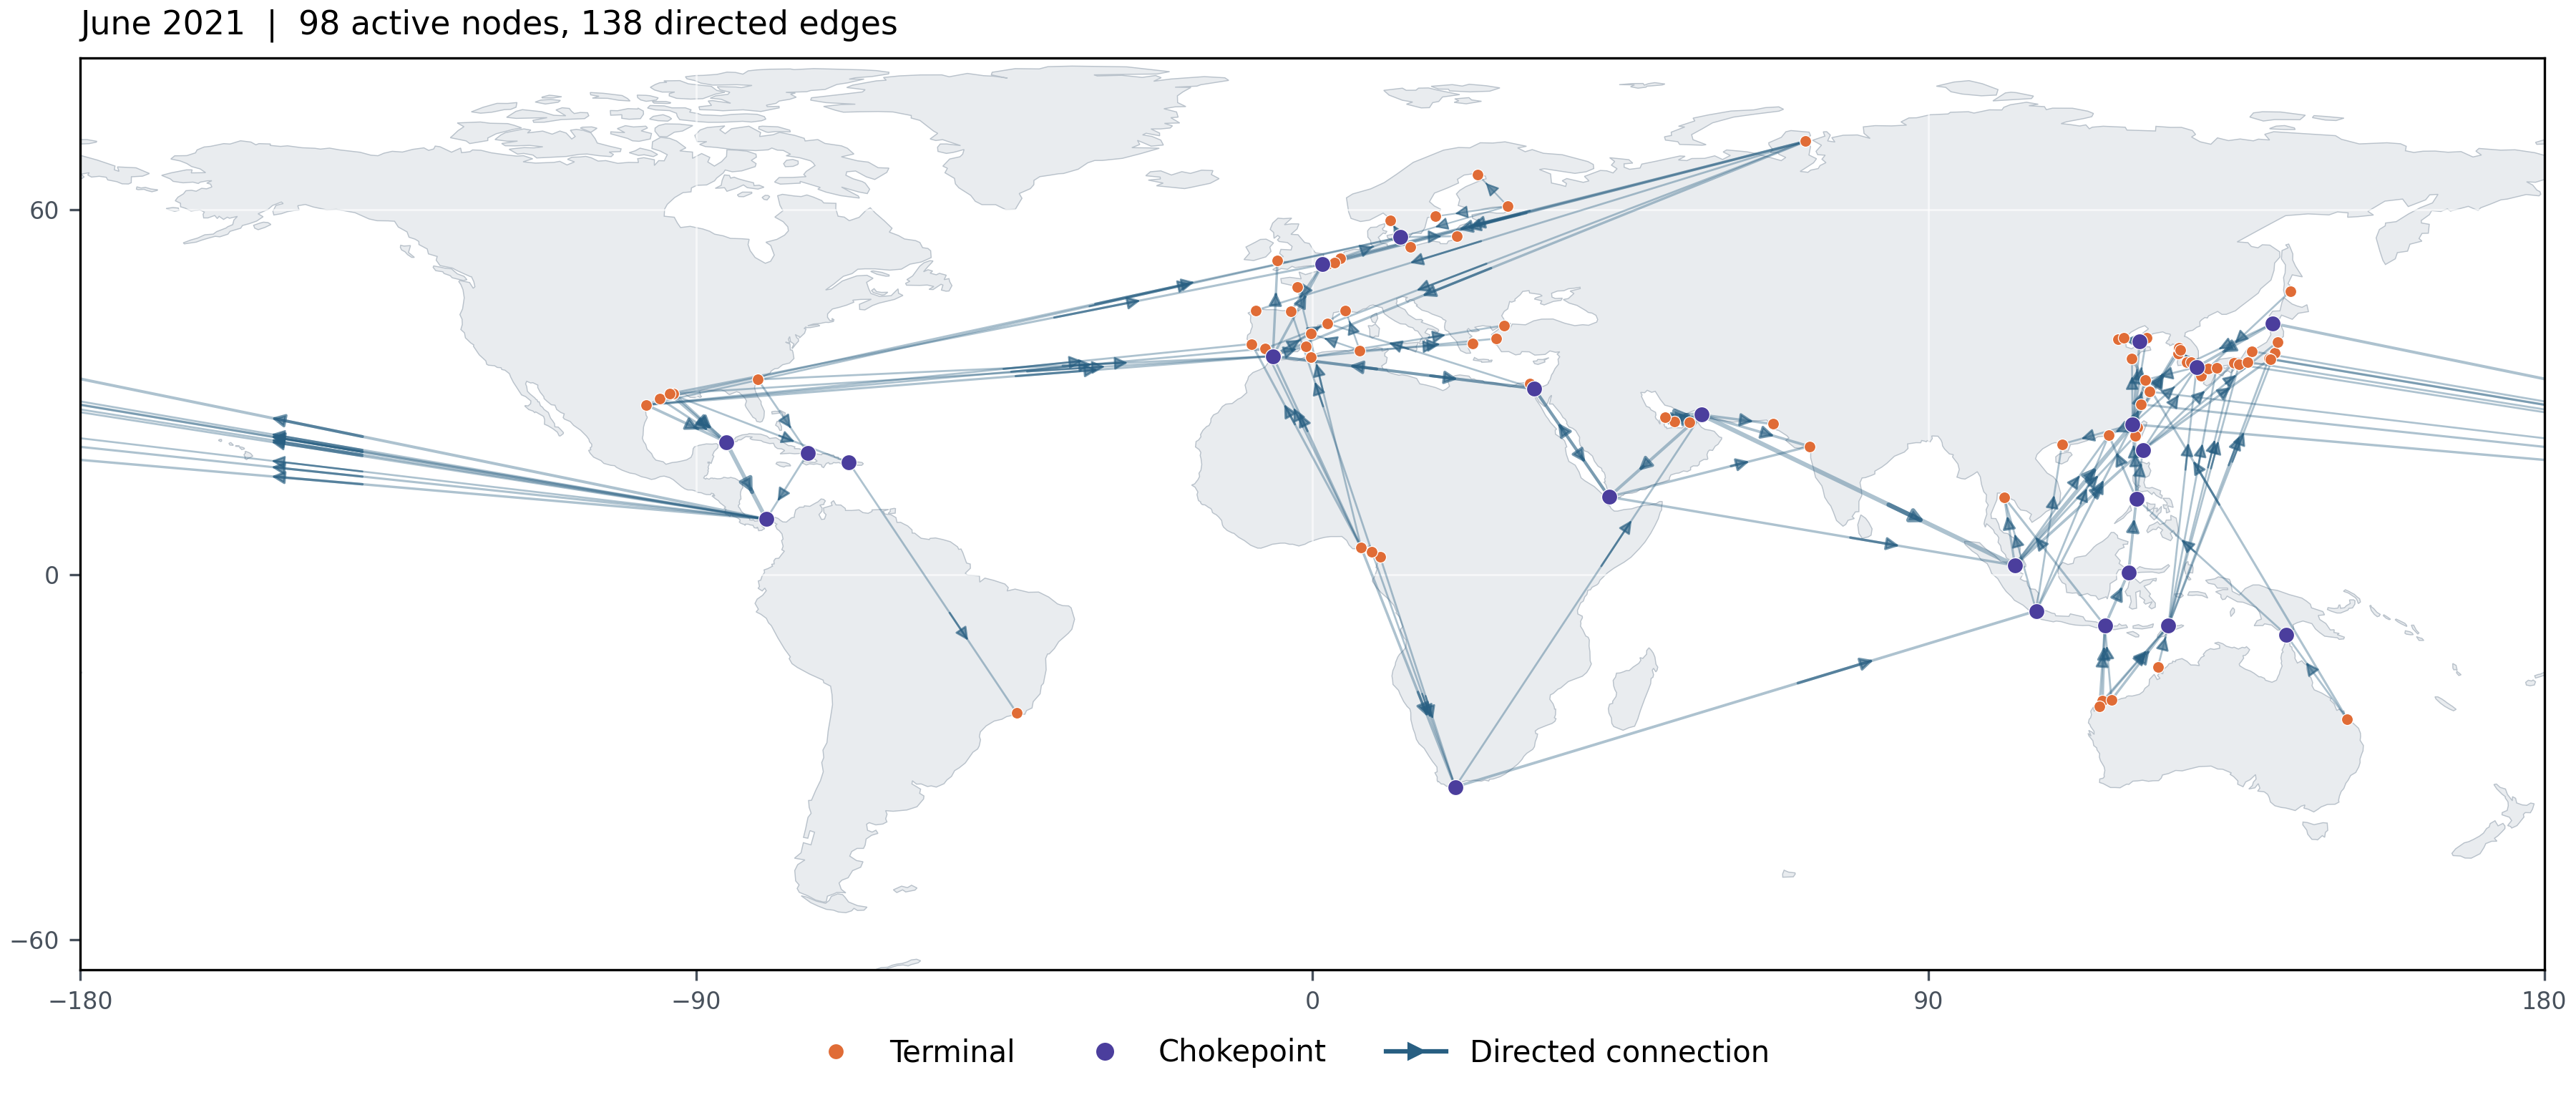
\includegraphics[width=\textwidth]{images/lng_network_2021-06.png}
    \caption{Geographic snapshot of the observed LNG network in June 2021.
    Points show active terminals and chokepoints; arrows indicate the
    direction of observed network connections. 
    Line width represents monthly LNG volume on each directed edge; connections are schematic rather than sailed routes.}
    \label{fig:lng_network_june2021}
\end{figure}

Figure~\ref{fig:eda_export_volume} shows how observed LNG export volume
changes from month to month, complementing the range and average reported
in the table. 
The increase in observed export volume through 2023 is consistent with
the growth in global LNG trade reported by the U.S. Energy Information
Administration \citep{eia2024lng}. This comparison provides context for
the overall pattern but does not explain individual monthly fluctuations.

\begin{figure}[H]
  \centering
  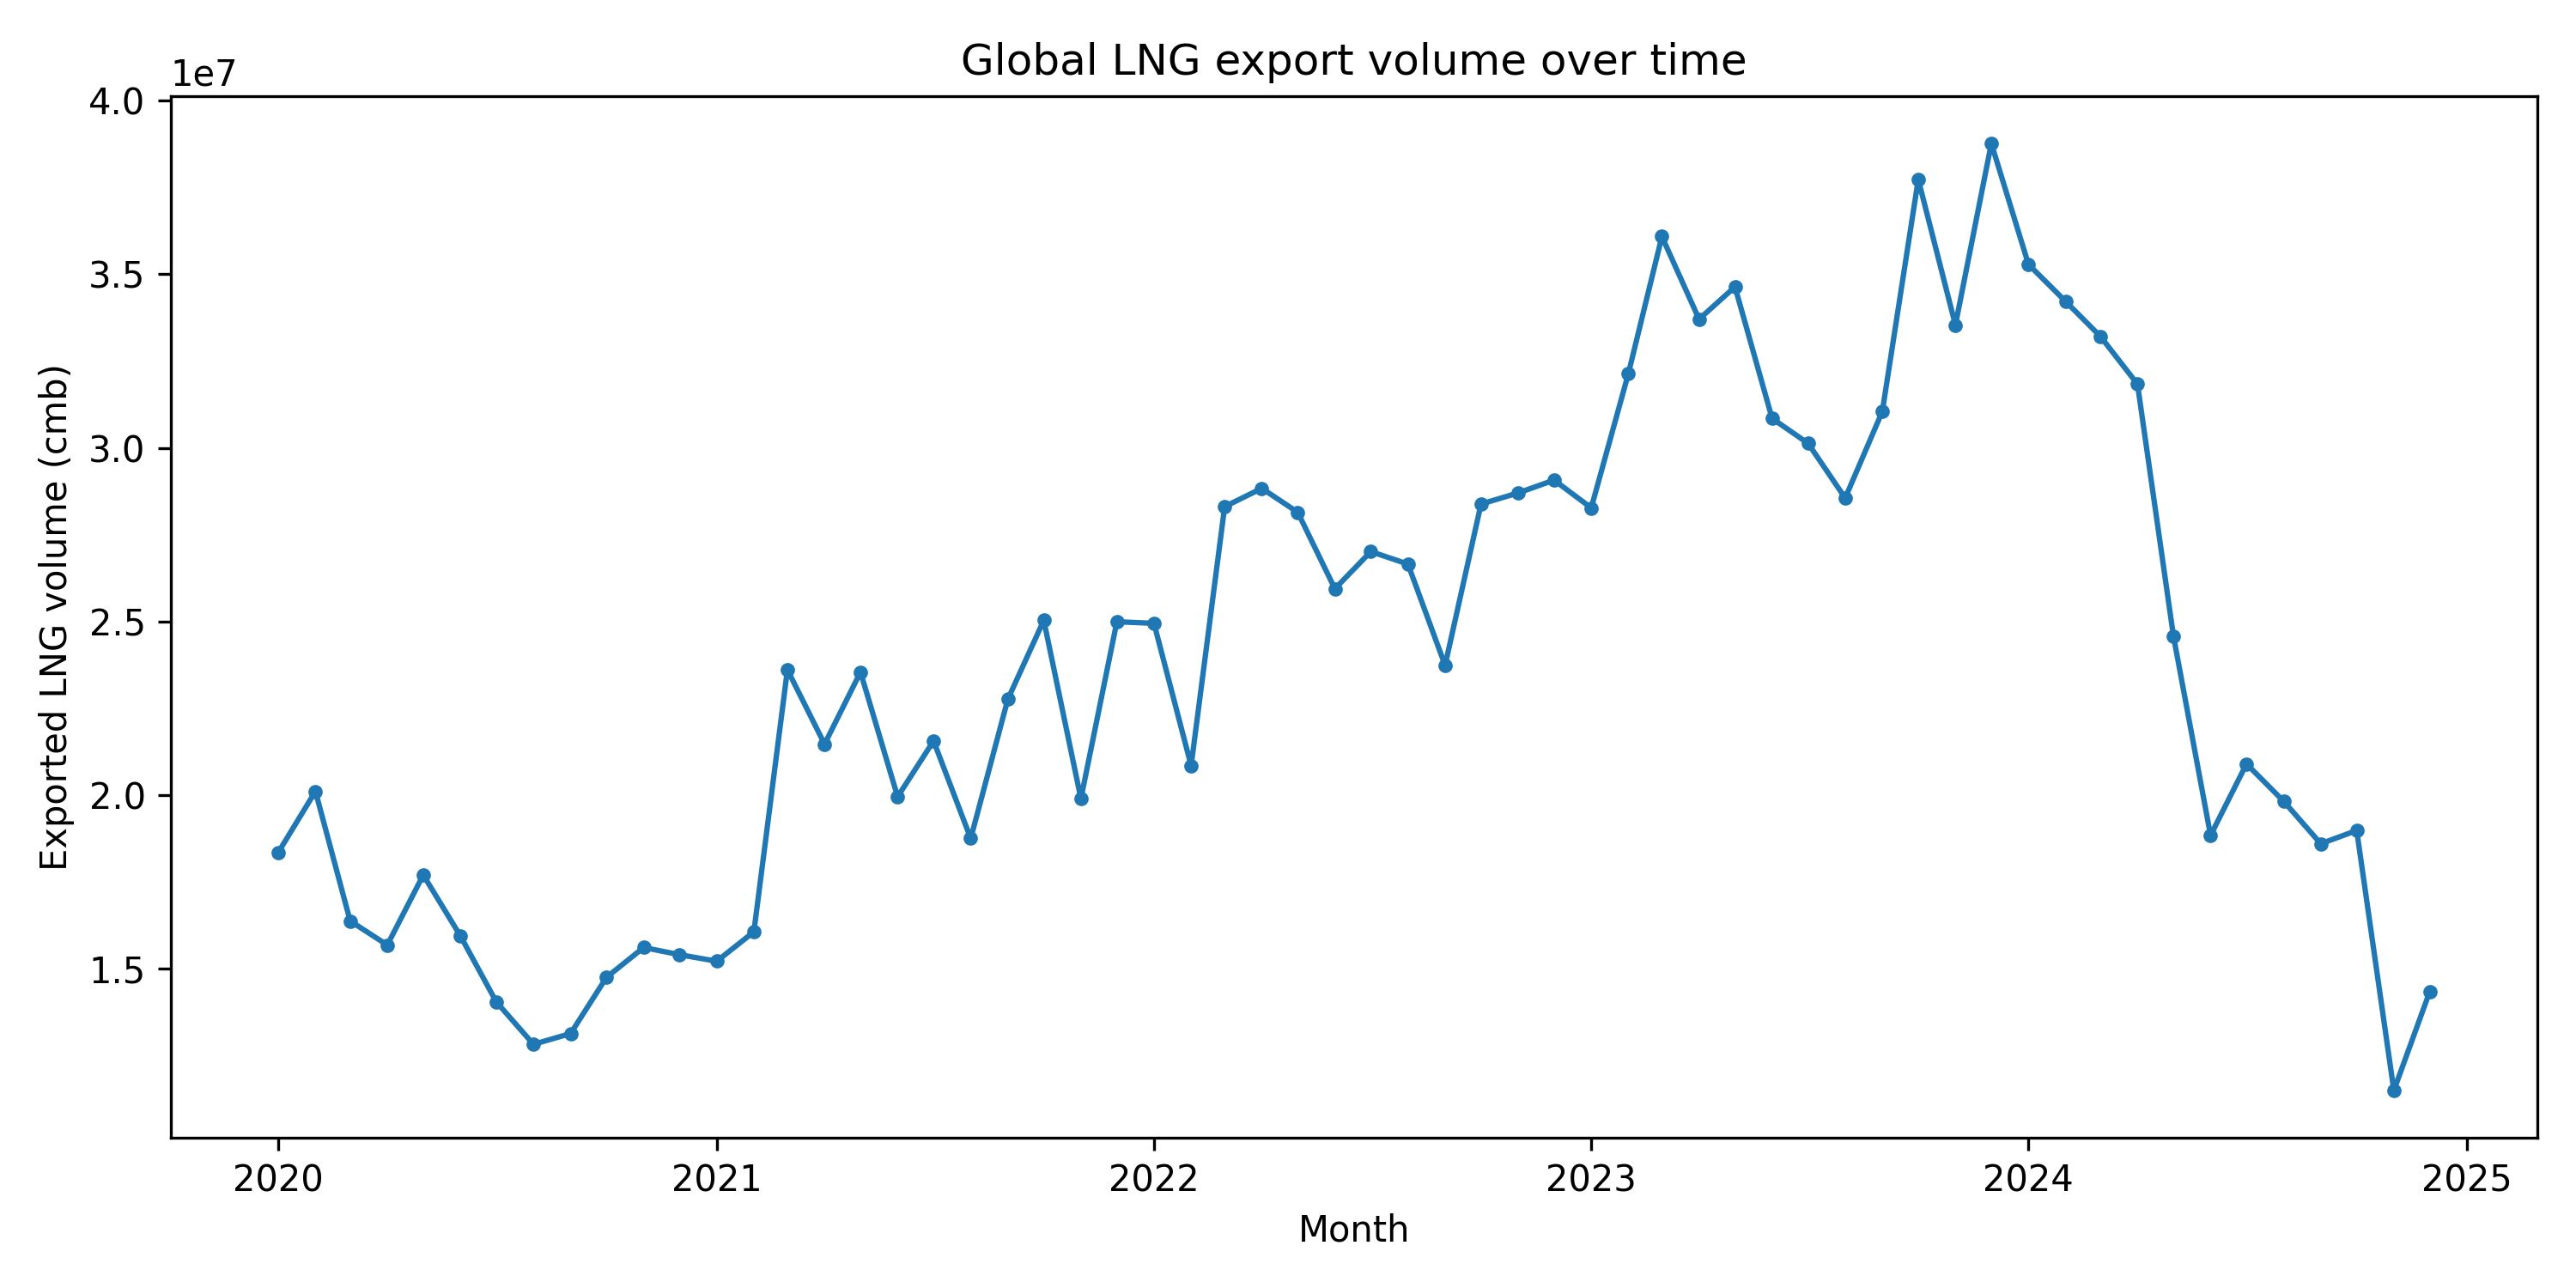
\includegraphics[width=.82\textwidth]{images/global_lng_export_volume_over_time.png}
  \caption{Monthly LNG export volume based on observed export voyages (cubic metres).}
  \label{fig:eda_export_volume}
\end{figure}

Changes in the numbers of nodes and edges, and in exported volume, do not
show whether active nodes belong to the same connected part of the network.
To examine this aspect, the weakly connected components of each
monthly graph were considered. The monthly graph is not always weakly connected, although
its largest weakly connected component contains at least 89.8\% of active
nodes throughout the period. Thus, most active nodes belong to one component
even when smaller components exist. 

\section{Node activity and temporal sparsity}
\label{sec:activity_sparsity}

Using the node activity definition introduced in Chapter~\ref{subsec:node_activity_definition}, of 10,980 potential node-month observations, 5,792 (52.75\%) are active and 5,188 (47.25\%) inactive. 
Consistent with the broad pattern in exported LNG volume shown in Figure~\ref{fig:eda_export_volume}, node participation generally increases through 2023 and declines towards the end of 2024. 
Correspondingly, the monthly share of inactive nodes ranges from 31.15\% to 60.66\% (Figure~\ref{fig:eda_sparsity}).

Terminals account for 9,540 node--month observations, of which 4,552 are
active and 4,988 inactive (52.29\%). The 24 chokepoints account
for 1,440 observations, of which 1,240 are active and 200 inactive
(13.89\%). This difference is consistent with the nodes'
distinct roles in the network: a terminal participates as an origin or
destination of a voyage, whereas a chokepoint can be traversed by voyages
linking many different terminal pairs. Aggregate inactivity is therefore
predominantly a terminal phenomenon, although chokepoint activity is not
constant. These different base rates suggest that activity may need to be
examined separately by node type.

\begin{figure}[htbp]
  \centering
  
\includegraphics[width=.85\textwidth]{images/monthly_sparsity_over_time.png}
  \caption{Monthly inactive-node shares for all nodes and by node type.}
  \label{fig:eda_sparsity}
\end{figure}

Inactivity is substantively relevant to the interpretation of centrality: an inactive node may receive a zero in the balanced node-month dataset even though the criticality measure is chiefly meaningful when it participates in trade. 
A later activity component can therefore address participation separately from the magnitude of criticality conditional on activity.
The descriptive shares support examining such a specification.

\section{Terminal activity and network position}
\label{sec:terminal_trade_patterns}
This section examines how terminals participate in observed LNG trade
and how their positions differ across the monthly networks. It first
describes terminal roles and operational activity, then considers
centrality, counterparty concentration, dependence, and structural
position.

\subsection{Terminal roles and operational activity}
\label{subsec:terminal_roles_eda}
Terminal participation is uneven across the 60 monthly networks.
Of the 9,540 terminal--month observations, 3,234 are active importer months, 1,318 are active exporter months, and 4,988 are inactive months.

Country-level roles were assessed over the full 2020--2024 period using each country's net trade position. 
Qatar, the United States, and Russia recorded the largest cumulative export volumes, while China, France, and Japan recorded the largest cumulative import volumes. 
A net role does not imply trade in only one direction: Malaysia was a net importer despite recording exports, and the United States was a net exporter despite recording imports.

Table~\ref{tab:eda_terminal_activity_by_role} compares throughput, voyage counts, and numbers of terminal counterparties across active importer and exporter months. 
Exporter observations have higher medians and 95th percentiles for all three measures. 
For example, median monthly throughput is approximately 0.505 million cubic metres for exporters and 0.328 million cubic metres for importers.

\begin{table}[htbp]
    \centering
    \caption{Operational activity of active terminal--month observations
    by terminal role, 2020--2024.}
    \label{tab:eda_terminal_activity_by_role}
    \begin{tabular}{lrrrr}
        \hline
        & \multicolumn{2}{c}{Importer ($n=3{,}234$)}
        & \multicolumn{2}{c}{Exporter ($n=1{,}318$)} \\
        \cline{2-3} \cline{4-5}
        Measure & Median & 95th percentile & Median & 95th percentile \\
        \hline
        Throughput (million cubic metres) & 0.328 & 1.226 & 0.505 & 3.792 \\
        Voyages & 2 & 7 & 4 & 22 \\
        Terminal counterparties & 1 & 4 & 3 & 14 \\
        \hline
    \end{tabular}
    \begin{flushleft}
        \footnotesize Source: calculations from
        \texttt{terminal\_month\_metrics.csv}, restricted to active
        terminal--month observations and grouped by terminal role.
        Throughput values are rounded to three decimal places.
    \end{flushleft}
\end{table}

Across all active terminal--month observations, median throughput
is 346,000 cubic metres, but its distribution is highly right-skewed: the 95th
percentile is approximately 1.90 million cubic metres, while Rasgas LNG Terminal 3 reaches the observed maximum of 10.91 million cubic metres in October 2023. 
This skew motivates considering a transformation of lagged throughput in the subsequent modelling analysis.

The differences in voyage counts and counterparties in Table~\ref{tab:eda_terminal_activity_by_role} also show that monthly terminal activity varies beyond traded volume. 
Active exporter terminal--months involve more terminal counterparties than active importer terminal--months, with respective medians of three and one, which suggests greater diversification of observed trading connections among exporters. 

\subsection{Centrality, concentration and dependence}
\label{subsec:terminal_criticality_eda}
The terminal measures discussed below were defined in Section~\ref{subsec:terminal_measures}. Here, their distributions are examined across active terminal--month observations.

Role-specific PageRank has a median of 0.0142 and a 95th percentile of 0.0363. 
Its distribution is clearly right-skewed, as most observations have relatively low values, while a small number attain substantially higher PageRank. 
Whereas this is a signal of variation in measured network position, a high PageRank alone does not establish a node's criticality in the network. 
For this reason, the following measures were evaluated to describe other dimensions of its role in the network.

The counterparty concentration measures show substantial variation
among active terminal--month observations. The median HHI is 0.556
when counterparties are individual terminals and 0.674 when they
are aggregated by country. These values correspond to effective
numbers of approximately 1.8 terminals and 1.5 countries,
respectively. Thus, even when a terminal trades with several
partners, its observed monthly flow may be concentrated among
relatively few of them.

An HHI of one occurs in 43.5\% of active terminal--month
observations at the terminal level, meaning that all role-relevant
flow observed in that month involves a single terminal counterparty.
At the country level, the corresponding share is 47.4\%: all
role-relevant flow goes to or comes from one country, which may
contain multiple terminal counterparties.

Role-specific dependence has a median of 0.406 across active
terminal--month observations, but this pooled value combines
different interpretations for the two terminal roles. Among active
exporter months, the median is 0.495: higher values indicate that
a larger share of the exporter's flow reaches importing terminals
that rely heavily on its supply. 
Among active importer months instead, where higher values indicate that the terminal
accounts for a larger share of its country's observed LNG receipts, the median is 0.333.

The two role-specific values refer to different forms of reliance.
For an exporter, dependence describes how strongly its importing
terminal counterparties rely on its supply. For an importer, it
describes how much of its country's observed LNG receipts pass
through that terminal. Their numerical values therefore should
not be interpreted as measuring the same relationship.

Counterparty HHI captures yet another aspect of trade relationships:
the concentration of a terminal's own trade across its partners.
An importer may receive all its LNG from one exporter, giving it
an HHI of one, while handling only a small share of its country's
total imports and therefore having low role-specific dependence.

Both measures are therefore retained to describe complementary
aspects of a terminal's role in the trade network.

\subsection{Structural position}
\label{subsec:terminal_structure}

The monthly undirected projection provides complementary binary indicators: whether a terminal is an articulation point, whether it is incident to a global bridge or to a local bridge that is not global, and whether it is adjacent to an articulation point. 
They reflect connectivity and exposure to fragile connections rather than trade volume. 
These indicators can be discussed alongside centrality and dependence, without treating them as interchangeable. 
For terminals, shortest-path betweenness in the directed monthly network is identically zero in the published node-month summary and consequently offers no variation for a terminal criticality outcome.

\section{Chokepoint criticality}
\label{sec:chokepoint_criticality_measures}

Chokepoints are transit nodes. Their throughput is calculated as one half of incoming plus outgoing segment flow, so that cargo passing through a chokepoint is counted once. Relative to total \emph{original-voyage} exported volume in a month, this gives the chokepoint's share of monthly network flow. Shares across different chokepoints need not sum to one, because a voyage may cross multiple passages. Across all 1,440 chokepoint-months, including inactive months, the median flow share is 0.0125 and the 95th percentile is 0.0607.

Weighted betweenness uses shortest paths on the directed monthly graph with edge distance equal to inverse positive LNG flow. It therefore measures intermediation on the graph's flow-weighted shortest paths, not the fraction of actual reconstructed voyages through a passage. Its median across chokepoint-months is 0.0060; zero values can also occur in active months. Chokepoint PageRank, computed on the directed graph with flow weights, has a median of 0.0151. The three quantities describe different facets of passage importance, but their common dependence on observed network use means that empirical association is expected.

The structural bridge and articulation indicators add a different question: whether removal of a node or an incident connection changes local or global connectivity in the undirected projection. These measures are valuable precisely because a passage can have high traffic without being a unique connector, and conversely a lower-volume connection can be structurally important. They should be interpreted with the monthly active graph and its component structure in mind.

\section{Associations and modelling implications}
\label{sec:associations_variable_selection}

Spearman rank correlations provide a preliminary check for overlap among observed measures. In the all-month terminal node panel, throughput and voyage count correlate at 0.989, throughput and total route exposure at 0.980, and throughput and flow share at 0.992. For chokepoints the corresponding throughput--voyage and throughput--flow-share correlations are 0.995 and 0.972. Shared zero months contribute to these pooled associations; the coefficients are descriptive rather than evidence of a causal relationship or identical information conditional on activity.

Within active terminal roles, throughput is positively associated with voyage count (Spearman $0.922$ for exporters and $0.919$ for importers) and negatively associated with terminal-level counterparty HHI ($-0.913$ and $-0.749$, respectively). The relationship between throughput and role-specific PageRank differs by role ($0.764$ for exporters, $0.267$ for importers). These comparisons reinforce the need to retain role-specific interpretations and to distinguish scale from concentration or centrality. For chokepoints, betweenness and flow share correlate at 0.878, while PageRank and flow share correlate at 0.810; both are associated with, but do not have the same definition as, traffic exposure.

These patterns suggest a parsimonious preliminary separation of (i) a node-activity response, (ii) terminal criticality responses conditional on their meaningful support, and (iii) chokepoint criticality responses. Potential predictors include suitably lagged activity and operational scale, with $\log(1+x)$ transformations for nonnegative skewed variables. Throughput, voyage count, degree, route exposure and flow share should not all enter an unregularised equation as if they were independent sources of information. Equally, inverse HHI and HHI should not both be used as separate outcomes in the same interpretation. Reduced-rank modelling can capture shared structure across multiple responses, but it does not make duplicate or conceptually overlapping predictors informative.

The exact response set, handling of inactive-month zeros, link functions and dependence structure remain modelling decisions for Chapter~\ref{chap:bayesian_framework}. This chapter establishes the empirical reasons to examine separate node types and an activity component; it does not claim that an exploratory association identifies an effect.

%
%			CHAPTER 5: Bayesian modelling framework
%
\chapter{Bayesian modelling framework}
\label{chap:bayesian_framework}
% TODO: Complete after fixing the final model specification, priors, and
% posterior-computation strategy.

%
%			CHAPTER 6: Results and discussion
%
\chapter{Results and discussion}
\label{chap:results}
% TODO: Present activity, terminal-criticality, and chokepoint-criticality
% results, posterior diagnostics, sensitivity analyses, and discussion.

%
%			CHAPTER 7: Conclusions and future work
%
\chapter{Conclusions and future work}
\label{chap:conclusions}
% 
%			Appendix
% 
\appendix
\counterwithin{table}{chapter}

\chapter{Sensitivity analysis of chokepoint assignments}
\label{app:chokepoint_sensitivity}

\section{Purpose and method}

The identification of the chokepoints traversed by each reconstructed maritime
route may be affected by small spatial discrepancies between the
\texttt{SeaRoute} paths and the operational chokepoint geometries. Such
discrepancies can arise from the spatial resolution and simplification of the
routing network, the geographic representation adopted for each passage, and
small differences between a reconstructed route centreline and the
corresponding transit geometry.

A sensitivity analysis was therefore conducted to quantify how the
route--chokepoint assignments changed under alternative spatial specifications. Four classifications were compared: exact geometric
intersection and intersections obtained after applying uniform buffers of 5,
10, and 25~km around each of the 28 candidate chokepoint geometries. The
25-km specification corresponds to the classification retained for the final
network.

For each chokepoint, distances and buffers were calculated in a local
azimuthal-equidistant projection centred on the geometry, allowing the tolerance distance to be measured in metres rather than in geographic degrees. 
Each of the 1,037 reconstructed origin--destination routes
was then compared with the original and buffered chokepoint geometries. For
every route--chokepoint pair, the analysis recorded the minimum geometric
distance, exact-intersection status, and whether the route fell within each
alternative tolerance. The same tolerance was applied to every candidate
chokepoint, thereby avoiding passage-specific adjustments based on the
observed routes.

\section{Sensitivity results}

Table~\ref{tab:chokepoint_sensitivity} reports, for each candidate
chokepoint, the number of reconstructed routes identified through exact
intersection and under the three alternative tolerance buffers. The final
column gives the number of assignments added by the 25-km specification
relative to exact intersection.

\begingroup
\small
\setlength{\tabcolsep}{4pt}

\begin{longtable}{
    @{}
    >{\raggedright\arraybackslash}p{0.28\textwidth}
    >{\centering\arraybackslash}p{0.09\textwidth}
    >{\centering\arraybackslash}p{0.09\textwidth}
    >{\centering\arraybackslash}p{0.09\textwidth}
    >{\centering\arraybackslash}p{0.09\textwidth}
    >{\centering\arraybackslash}p{0.16\textwidth}
    @{}
}
\caption{Sensitivity of route--chokepoint assignments to alternative spatial tolerances}
\label{tab:chokepoint_sensitivity}\\

\toprule
\textbf{Chokepoint} &
\textbf{Exact} &
\textbf{5 km} &
\textbf{10 km} &
\textbf{25 km} &
\textbf{Additional at 25 km} \\
\midrule
\endfirsthead

\multicolumn{6}{l}{\tablename\ \thetable\ continued}\\
\toprule
\textbf{Chokepoint} &
\textbf{Exact} &
\textbf{5 km} &
\textbf{10 km} &
\textbf{25 km} &
\textbf{Additional at 25 km} \\
\midrule
\endhead

\midrule
\multicolumn{6}{r}{Continued on next page}\\
\endfoot

\bottomrule
\endlastfoot

Suez Canal             & 151 & 151 & 151 & 151 & 0  \\
Panama Canal           & 148 & 148 & 148 & 148 & 0  \\
Bosporus Strait        & 0   & 0   & 0   & 0   & 0  \\
Bab el-Mandeb Strait   & 147 & 147 & 147 & 147 & 0  \\
Malacca Strait         & 133 & 133 & 133 & 133 & 0  \\
Strait of Hormuz       & 122 & 122 & 122 & 122 & 0  \\
Cape of Good Hope      & 65  & 65  & 65  & 65  & 0  \\
Gibraltar Strait       & 216 & 222 & 222 & 222 & 6  \\
Dover Strait           & 91  & 91  & 91  & 91  & 0  \\
Oresund Strait         & 47  & 47  & 47  & 47  & 0  \\
Taiwan Strait          & 152 & 152 & 152 & 152 & 0  \\
Korea Strait           & 3   & 3   & 3   & 68  & 65 \\
Tsugaru Strait         & 50  & 50  & 52  & 52  & 2  \\
Luzon Strait           & 43  & 56  & 56  & 56  & 13 \\
Lombok Strait          & 69  & 69  & 69  & 74  & 5  \\
Ombai Strait           & 57  & 57  & 57  & 58  & 1  \\
Bohai Strait           & 35  & 35  & 35  & 35  & 0  \\
Torres Strait          & 5   & 5   & 5   & 5   & 0  \\
Sunda Strait           & 51  & 51  & 51  & 51  & 0  \\
Makassar Strait        & 58  & 58  & 58  & 58  & 0  \\
Magellan Strait        & 2   & 2   & 2   & 2   & 0  \\
Yucatan Channel        & 137 & 137 & 137 & 137 & 0  \\
Windward Passage       & 10  & 10  & 10  & 10  & 0  \\
Mona Passage           & 17  & 17  & 17  & 17  & 0  \\
Balabac Strait         & 0   & 0   & 0   & 0   & 0  \\
Bering Strait          & 0   & 0   & 0   & 0   & 0  \\
Mindoro Strait         & 0   & 0   & 8   & 63  & 63 \\
Kerch Strait           & 0   & 0   & 0   & 0   & 0  \\
\midrule
\textbf{Total assignments} & \textbf{1,809} & \textbf{1,828} &
\textbf{1,838} & \textbf{1,964} & \textbf{155} \\
\textbf{Observed chokepoints} & \textbf{23} & \textbf{23} &
\textbf{24} & \textbf{24} & --- \\

\end{longtable}
\endgroup

Exact intersection identified 1,809 route--chokepoint assignments involving
23 of the 28 candidate passages. Under the final 25-km specification, the
number of assignments increased to 1,964 and the number of identified
chokepoints increased to 24, resulting in 155 additional assignments, or
an 8.6\% increase relative to exact intersection.

The assignments were stable across all four specifications for 17 of the 24 chokepoints retained in the final network. 
Most of the additional assignments under the final specification were concentrated in Korea Strait and Mindoro Strait, indicating that the results for these two passages were particularly sensitive to the selected spatial tolerance.

Four candidate chokepoints---Bosporus Strait, Balabac Strait, Bering Strait,
and Kerch Strait---were not traversed under any of the evaluated
specifications: their minimum distances from the closest reconstructed routes
were approximately 71.3, 162.0, 2,617.3, and 829.7~km, respectively. They were
therefore excluded from the final monthly network. The exclusion indicates
that none of the reconstructed LNG routes in the study period passed within
25~km of their operational geometries, but it does not imply that the passages
have no relevance to maritime traffic outside the analysed LNG network.

\section{Selection of the final specification}

The 25-km tolerance was retained because it accommodates spatial
misalignments between the simplified \texttt{SeaRoute} paths and the
operational transit geometries while applying a uniform and transparent
classification rule to all candidate passages. The exact-intersection
assignments were preserved separately for reproducibility, and the sensitivity
procedure did not alter the reconstructed route geometries.


\chapter{Model-ready panels variables}
\label{app:model_ready_variables}

This appendix documents the variables contained in the three model-ready panels described in Section~\ref{sec:model_ready_panels}. 
Variables are grouped according to their analytical role rather than their physical order in the CSV files. 
Flow variables are measured monthly, binary indicators take the value one when the stated condition is satisfied, and variables carrying the suffix \texttt{lag1} refer to month (t-1).
Log-transformed variables were calculated using \(\log(1+x)\).

The three panels cover January 2020--December 2024. Consequently, all one-month lagged variables are unavailable in January 2020. 
Measures based on historical neighbours are additionally unavailable until a node has acquired at least one neighbour through a connection observed before the current month. 
Commercial criticality measures that require realised trade are defined only for active terminal--months.

\section{Node activity panel}

\begingroup
\small
\setlength{\tabcolsep}{4pt}

\begin{longtable}{>{\raggedright\arraybackslash}p{0.27\textwidth}
                  >{\raggedright\arraybackslash}p{0.52\textwidth}
                  >{\raggedright\arraybackslash}p{0.13\textwidth}}
\caption{Variables in the node activity panel}\label{tab:activity_panel_variables}\\
\toprule
\textbf{Variable} & \textbf{Definition} & \textbf{Role} \\
\midrule
\endfirsthead

\multicolumn{3}{l}{\tablename\ \thetable\ continued}\\
\toprule
\textbf{Variable} & \textbf{Definition} & \textbf{Role} \\
\midrule
\endhead

\midrule
\multicolumn{3}{r}{Continued on next page}\\
\endfoot

\bottomrule
\endlastfoot

\path{node_id} & Unique node identifier. & Identifier \\
\path{period_month} & Calendar month of observation. & Identifier \\
\path{node_name} & Node name. & Identifier \\
\path{node_type} & Node category: terminal or chokepoint. & Covariate \\
\path{country} & Country in which a terminal is located; not applicable to chokepoints. & Covariate \\
\path{active} & Equals one when the node participates in the monthly network and zero otherwise. & Outcome \\
\path{incoming_flow} & Total LNG volume entering the node in month (t). & Descriptive \\
\path{outgoing_flow} & Total LNG volume leaving the node in month (t). & Descriptive \\
\path{incident_flow} & Sum of incoming and outgoing LNG volume incident to the node. & Descriptive \\
\path{node_throughput} & Node throughput, adjusted for double counting at chokepoints. & Descriptive \\
\path{in_degree} & Number of distinct incoming neighbours in the monthly directed network. & Descriptive \\
\path{out_degree} & Number of distinct outgoing neighbours in the monthly directed network. & Descriptive \\
\path{total_degree} & Sum of monthly in-degree and out-degree. & Descriptive \\
\path{in_voyages} & Number of incoming voyage movements associated with the node. & Descriptive \\
\path{out_voyages} & Number of outgoing voyage movements associated with the node. & Descriptive \\
\path{incident_voyage_traversals} & Sum of incoming and outgoing voyage traversals incident to the node. & Descriptive \\
\path{total_voyages} & Number of voyages associated with the node, adjusted for double counting at chokepoints. & Descriptive \\
\path{in_route_exposure} & Number of reconstructed routes entering the node. & Descriptive \\
\path{out_route_exposure} & Number of reconstructed routes leaving the node. & Descriptive \\
\path{total_route_exposure} & Total reconstructed-route exposure of the node. & Descriptive \\
\path{betweenness} & Normalised weighted betweenness centrality in the monthly segment-level network. & Descriptive \\
\path{pagerank} & Weighted PageRank in the monthly directed segment-level network. & Descriptive \\
\path{share_monthly_network_flow} & Share of total monthly node throughput associated with the node. & Descriptive \\
\path{months_since_last_active} & Number of months elapsed since the node was last active; unavailable before its first observed active month. & Supplementary \\
\path{infrastructure_type} & Terminal infrastructure role, classified as import or export; not applicable to chokepoints. & Covariate \\
\path{capacity_mtpa} & Annual terminal processing capacity in million tonnes per annum; not applicable to chokepoints. & Covariate \\
\path{log1p_capacity_mtpa} & Log-transformed annual terminal processing capacity. & Covariate \\
\path{start_year} & Year in which the terminal began operating; not applicable to chokepoints. & Covariate \\
\path{activity_lag1} & Activity status in the preceding month. & Covariate \\
\path{throughput_lag1} & Node throughput in the preceding month. & Covariate \\
\path{log1p_throughput_lag1} & Log-transformed node throughput in the preceding month. & Covariate \\
\path{voyage_count_lag1} & Number of voyages associated with the node in the preceding month. & Covariate \\
\path{log1p_voyage_count_lag1} & Log-transformed voyage count in the preceding month. & Covariate \\
\path{historical_neighbor_count_lag1} & Number of neighbours connected to the node by at least one edge observed up to (t-1). & Covariate \\
\path{active_neighbor_count_lag1} & Number of historical neighbours active in (t-1). & Covariate \\
\path{neighbor_activity_lag1} & Share of historical neighbours active in (t-1). & Covariate \\
\path{lag_available} & Equals one when preceding-month values can be calculated and zero in January 2020. & Availability \\
\path{year} & Calendar year. & Time index \\
\path{month} & Calendar month, coded from 1 to 12. & Time index \\
\path{month_sin} & Sine transformation of the calendar month. & Covariate \\
\path{month_cos} & Cosine transformation of the calendar month. & Covariate \\

\end{longtable}
\endgroup

\section{Terminal criticality panel}

\begingroup
\small
\setlength{\tabcolsep}{4pt}

\begin{longtable}{>{\raggedright\arraybackslash}p{0.27\textwidth}
                  >{\raggedright\arraybackslash}p{0.52\textwidth}
                  >{\raggedright\arraybackslash}p{0.13\textwidth}}
\caption{Variables in the terminal criticality panel}\label{tab:terminal_panel_variables}\\
\toprule
\textbf{Variable} & \textbf{Definition} & \textbf{Role} \\
\midrule
\endfirsthead
\multicolumn{3}{l}{\tablename\ \thetable\ continued}\\
\toprule
\textbf{Variable} & \textbf{Definition} & \textbf{Role} \\
\midrule
\endhead
\midrule
\multicolumn{3}{r}{Continued on next page}\\
\endfoot
\bottomrule
\endlastfoot

\path{terminal_id} & Unique terminal identifier. & Identifier \\
\path{node_name} & Terminal name. & Identifier \\
\path{period_month} & Calendar month of observation. & Identifier \\
\path{year} & Calendar year. & Time index \\
\path{month} & Calendar month, coded from 1 to 12. & Time index \\
\path{node_type} & Node category, equal to terminal throughout this panel. & Descriptor \\
\path{country} & Country in which the terminal is located. & Covariate \\
\path{infrastructure_type} & Terminal infrastructure role, classified as import or export. & Covariate \\
\path{capacity_mtpa} & Annual processing capacity in million tonnes per annum. & Covariate \\
\path{log1p_capacity_mtpa} & Log-transformed annual processing capacity. & Covariate \\
\path{unit_count} & Number of infrastructure units associated with the terminal. & Covariate \\
\path{start_year} & Year in which the terminal began operating. & Covariate \\
\path{terminal_age} & Difference between the observation year and the terminal start year; unavailable before the start year. & Covariate \\
\path{terminal_role} & Observed monthly role: exporter, importer, or inactive. & Descriptor \\
\path{active} & Equals one when the terminal participates in LNG trade in month (t). & Conditioning indicator \\
\path{export_share} & Share of terminal throughput represented by outgoing flow; defined for active terminal--months. & Descriptor \\
\path{outgoing_flow} & Total LNG volume exported by the terminal. & Descriptive \\
\path{incoming_flow} & Total LNG volume imported by the terminal. & Descriptive \\
\path{throughput} & Sum of outgoing and incoming LNG volume. & Descriptive \\
\path{outgoing_voyages} & Number of voyages departing from the terminal. & Descriptive \\
\path{incoming_voyages} & Number of voyages arriving at the terminal. & Descriptive \\
\path{voyage_count} & Total number of voyages associated with the terminal. & Descriptive \\
\path{counterparty_count} & Number of distinct terminal counterparties. & Descriptive \\
\path{counterparty_country_count} & Number of distinct counterparty countries. & Descriptive \\
\path{counterparty_hhi_terminal} & Role-specific HHI of flows across terminal counterparties. & Outcome \\
\path{counterparty_hhi_country} & Role-specific HHI of flows across counterparty countries. & Outcome \\
\path{effective_counterparties_terminal} & Effective number of terminal counterparties, calculated as the inverse of the terminal-level HHI. & Supplementary \\
\path{effective_counterparties_country} & Effective number of counterparty countries, calculated as the inverse of the country-level HHI. & Supplementary \\
\path{max_dependence_generated} & Maximum recipient dependence generated by an exporting terminal. & Supplementary \\
\path{weighted_dependence_generated} & Exporter-generated dependence weighted by the distribution of its outgoing flow. & Supplementary \\
\path{country_terminal_dependence} & Importing terminal's share of total LNG imports received by its country. & Supplementary \\
\path{role_specific_dependence} & Dependence measure selected according to the terminal's observed monthly role. & Outcome \\
\path{import_pagerank} & Weighted PageRank calculated in the observed direction of LNG flows. & Supplementary \\
\path{export_pagerank} & Weighted PageRank calculated after reversing the direction of LNG flows. & Supplementary \\
\path{role_specific_pagerank} & Directional PageRank selected according to the terminal's observed monthly role. & Outcome \\
\path{degree_undirected} & Degree in the undirected projection of the active monthly network. & Structural \\
\path{is_articulation_point} & Equals one when removal of the terminal increases the number of connected components. & Outcome \\
\path{global_bridge_count} & Number of global bridges incident to the terminal. & Structural \\
\path{global_bridge_share} & Share of incident undirected edges classified as global bridges. & Structural \\
\path{local_bridge_only_count} & Number of incident local bridges after excluding global bridges. & Structural \\
\path{local_bridge_only_share} & Share of incident undirected edges classified as local-only bridges. & Structural \\
\path{has_incident_global_bridge} & Equals one when the terminal is incident to at least one global bridge. & Outcome \\
\path{connected_to_articulation_point} & Equals one when the terminal is directly connected to an articulation point. & Outcome \\
\path{activity_lag1} & Terminal activity status in the preceding month. & Covariate \\
\path{throughput_lag1} & Terminal throughput in the preceding month. & Covariate \\
\path{log1p_throughput\_lag1} & Log-transformed terminal throughput in the preceding month. & Covariate \\
\path{voyage_count_lag1} & Terminal voyage count in the preceding month. & Covariate \\
\path{log1p_voyage_count_lag1} & Log-transformed terminal voyage count in the preceding month. & Covariate \\
\path{mean_voyage_distance_lag1} & Role-relevant mean voyage distance in the preceding month; undefined when no applicable voyage was observed. & Covariate \\
\path{log1p_mean_voyage_distance_lag1} & Log-transformed preceding-month role-relevant mean voyage distance, with structurally absent distances represented by zero. & Covariate \\
\path{historical_neighbor_count_lag1} & Number of historical neighbours observed up to (t-1). & Covariate \\
\path{active_neighbor_count_lag1} & Number of historical neighbours active in (t-1). & Covariate \\
\path{neighbor_activity_lag1} & Share of historical neighbours active in (t-1). & Covariate \\
\path{lag_available} & Equals one when preceding-month information can be calculated. & Availability \\
\path{month_sin} & Sine transformation of the calendar month. & Covariate \\
\path{month_cos} & Cosine transformation of the calendar month. & Covariate \\
\end{longtable}
\endgroup

\section{Chokepoint criticality panel}

\begingroup
\small
\setlength{\tabcolsep}{4pt}

\begin{longtable}{>{\raggedright\arraybackslash}p{0.27\textwidth}
                  >{\raggedright\arraybackslash}p{0.52\textwidth}
                  >{\raggedright\arraybackslash}p{0.13\textwidth}}
\caption{Variables in the chokepoint criticality panel}\label{tab:chokepoint_panel_variables}\\
\toprule
\textbf{Variable} & \textbf{Definition} & \textbf{Role} \\
\midrule
\endfirsthead
\multicolumn{3}{l}{\tablename\ \thetable\ continued}\\
\toprule
\textbf{Variable} & \textbf{Definition} & \textbf{Role} \\
\midrule
\endhead
\midrule
\multicolumn{3}{r}{Continued on next page}\\
\endfoot
\bottomrule
\endlastfoot

\path{node_id} & Unique chokepoint identifier. & Identifier \\
\path{period_month} & Calendar month of observation. & Identifier \\
\path{node_name} & Chokepoint name. & Identifier \\
\path{node_type} & Node category, equal to chokepoint throughout this panel. & Descriptor \\
\path{active} & Equals one when the chokepoint is traversed in month (t). & Conditioning indicator \\
\path{incoming_flow} & Total LNG volume entering the chokepoint. & Descriptive \\
\path{outgoing_flow} & Total LNG volume leaving the chokepoint. & Descriptive \\
\path{incident_flow} & Sum of incoming and outgoing LNG volume incident to the chokepoint. & Descriptive \\
\path{node_throughput} & Chokepoint throughput, equal to one half of incident flow. & Descriptive \\
\path{in_degree} & Number of distinct incoming neighbours. & Descriptive \\
\path{out_degree} & Number of distinct outgoing neighbours. & Descriptive \\
\path{total_degree} & Sum of directed in-degree and out-degree. & Descriptive \\
\path{in_voyages} & Number of incoming voyage traversals. & Descriptive \\
\path{out_voyages} & Number of outgoing voyage traversals. & Descriptive \\
\path{incident_voyage_traversals} & Sum of incoming and outgoing voyage traversals. & Descriptive \\
\path{total_voyages} & Chokepoint voyage count adjusted for double counting across incoming and outgoing segments. & Descriptive \\
\path{in_route_exposure} & Number of reconstructed routes entering the chokepoint. & Descriptive \\
\path{out_route_exposure} & Number of reconstructed routes leaving the chokepoint. & Descriptive \\
\path{total_route_exposure} & Total reconstructed-route exposure of the chokepoint. & Descriptive \\
\path{betweenness} & Normalised weighted betweenness centrality. & Outcome \\
\path{pagerank} & Weighted PageRank in the monthly directed segment-level network. & Outcome \\
\path{share_monthly_network_flow} & Share of total monthly node throughput associated with the chokepoint. & Outcome \\
\path{months_since_last_active} & Number of months since the chokepoint was last active; unavailable before its first active month. & Supplementary \\
\path{degree_undirected} & Degree in the undirected projection of the active monthly network. & Structural \\
\path{is_articulation_point} & Equals one when removal of the chokepoint increases the number of connected components. & Outcome \\
\path{global_bridge_count} & Number of global bridges incident to the chokepoint. & Structural \\
\path{global_bridge_share} & Share of incident undirected edges classified as global bridges. & Structural \\
\path{local_bridge_only_count} & Number of incident local bridges after excluding global bridges. & Structural \\
\path{local_bridge_only_share} & Share of incident undirected edges classified as local-only bridges. & Structural \\
\path{has_incident_global_bridge} & Equals one when the chokepoint is incident to at least one global bridge. & Outcome \\
\path{connected_to_articulation_point} & Equals one when the chokepoint is directly connected to an articulation point. & Outcome \\
\path{activity_lag1} & Chokepoint activity status in the preceding month. & Covariate \\
\path{throughput_lag1} & Chokepoint throughput in the preceding month. & Covariate \\
\path{log1p_throughput_lag1} & Log-transformed chokepoint throughput in the preceding month. & Covariate \\
\path{voyage_count_lag1} & Chokepoint voyage count in the preceding month. & Covariate \\
\path{log1p_voyage_count_lag1} & Log-transformed chokepoint voyage count in the preceding month. & Covariate \\
\path{historical_neighbor_count_lag1} & Number of historical neighbours observed up to (t-1). & Covariate \\
\path{active_neighbor_count_lag1} & Number of historical neighbours active in (t-1). & Covariate \\
\path{neighbor_activity_lag1} & Share of historical neighbours active in (t-1). & Covariate \\
\path{lag_available} & Equals one when preceding-month information can be calculated. & Availability \\
\path{year} & Calendar year. & Time index \\
\path{month} & Calendar month, coded from 1 to 12. & Time index \\
\path{month_sin} & Sine transformation of the calendar month. & Covariate \\
\path{month_cos} & Cosine transformation of the calendar month. & Covariate \\
\end{longtable}
\endgroup



\chapter{Data dictionary and supplementary descriptive results}
\label{app:data_dictionary}
% TODO: Add complete variable definitions and supplementary tables/figures.

\chapter{Model specification and diagnostics}
\label{app:model_diagnostics}
% TODO: Add priors, computational details, MCMC diagnostics, posterior
% predictive checks, and robustness analyses.

%
%			BIBLIOGRAPHY
%
\bibliography{references}
% 


\end{document}


 
